% concatenated from preprint.tex
\documentclass{article}

% if you need to pass options to natbib, use, e.g.:
%     \PassOptionsToPackage{numbers, compress}{natbib}
% before loading neurips_2026

% The authors should use one of these tracks.
% Before accepting by the NeurIPS conference, select one of the options below.
% 0. "default" for submission
\usepackage[preprint]{neurips_2026}
% the "default" option is equal to the "main" option, which is used for the Main Track with double-blind reviewing.
% 1. "main" option is used for the Main Track
%  \usepackage[main]{neurips_2026}
% 2. "position" option is used for the Position Paper Track
%  \usepackage[position]{neurips_2026}
% 3. "eandd" option is used for the Evaluations & Datasets Track
 % \usepackage[eandd]{neurips_2026}
 % if you need to opt-in for a single-blind submission in the E&D track:
 %\usepackage[eandd, nonanonymous]{neurips_2026}
% 4. "creativeai" option is used for the Creative AI Track
%  \usepackage[creativeai]{neurips_2026}
% 5. "sglblindworkshop" option is used for the Workshop with single-blind reviewing
 % \usepackage[sglblindworkshop]{neurips_2026}
% 6. "dblblindworkshop" option is used for the Workshop with double-blind reviewing
%  \usepackage[dblblindworkshop]{neurips_2026}

% After being accepted, the authors should add "final" behind the track to compile a camera-ready version.
% 1. Main Track
 % \usepackage[main, final]{neurips_2026}
% 2. Position Paper Track
%  \usepackage[position, final]{neurips_2026}
% 3. Evaluations & Datasets Track
 % \usepackage[eandd, final]{neurips_2026}
% 4. Creative AI Track
%  \usepackage[creativeai, final]{neurips_2026}
% 5. Workshop with single-blind reviewing
%  \usepackage[sglblindworkshop, final]{neurips_2026}
% 6. Workshop with double-blind reviewing
%  \usepackage[dblblindworkshop, final]{neurips_2026}
% Note. For the workshop paper template, both \title{} and \workshoptitle{} are required, with the former indicating the paper title shown in the title and the latter indicating the workshop title displayed in the footnote.
% For workshops (5., 6.), the authors should add the name of the workshop, "\workshoptitle" command is used to set the workshop title.
% \workshoptitle{WORKSHOP TITLE}

% "preprint" option is used for arXiv or other preprint submissions
 % \usepackage[preprint]{neurips_2026}

% to avoid loading the natbib package, add option nonatbib:
%    \usepackage[nonatbib]{neurips_2026}

\usepackage[utf8]{inputenc} % allow utf-8 input
\usepackage[T1]{fontenc}    % use 8-bit T1 fonts
\usepackage{hyperref}       % hyperlinks
\usepackage{url}            % simple URL typesetting
\usepackage{booktabs}       % professional-quality tables
\usepackage{amsfonts}       % blackboard math symbols
\usepackage{nicefrac}       % compact symbols for 1/2, etc.
\usepackage{microtype}      % microtypography
\usepackage{xcolor}         % colors
\usepackage{algorithm}
\usepackage[noend]{algorithmic}
% Note. For the workshop paper template, both \title{} and \workshoptitle{} are required, with the former indicating the paper title shown in the title and the latter indicating the workshop title displayed in the footnote. 
\usepackage{microtype}
\usepackage{graphicx}
\usepackage{subfigure} 
\usepackage{booktabs} % for professional tables
\usepackage{tikz}
\usetikzlibrary{arrows.meta}
% hyperref makes hyperlinks in the resulting PDF.
\usepackage{hyperref}

% Attempt to make hyperref and algorithmic work together better:

\usepackage{pgfplots}
\pgfplotsset{compat=1.17}


% For theorems and math
\usepackage{amsmath}
\usepackage{amssymb}
\usepackage{mathtools}
\usepackage{amsthm}
\usepackage{enumitem}
% if you use cleveref..
\usepackage[capitalize,noabbrev]{cleveref}

%%%%%%%%%%%%%%%%%%%%%%%%%%%%%%%%
% THEOREMS
%%%%%%%%%%%%%%%%%%%%%%%%%%%%%%%%
\theoremstyle{plain}
\newtheorem{theorem}{Theorem}[section]
\newtheorem{proposition}[theorem]{Proposition}
\newtheorem{lemma}[theorem]{Lemma}
\newtheorem{corollary}[theorem]{Corollary}
\theoremstyle{definition}
\newtheorem{definition}[theorem]{Definition}
\newtheorem{assumption}[theorem]{Assumption}
\theoremstyle{remark}
\newtheorem{remark}[theorem]{Remark}

% Custom Commands for RanSOM
\newcommand{\R}{\mathbb{R}}
\newcommand{\E}{\mathbb{E}}
\newcommand{\norm}[1]{\left\lVert#1\right\rVert}
\DeclareMathOperator{\LMO}{LMO}
\DeclareMathOperator{\argmin}{argmin}
\DeclareMathOperator{\Beta}{Beta}
\DeclareMathOperator{\Exp}{Exp}


\title{RanSOM: Second-Order Momentum with Randomized Scaling for Constrained and Unconstrained Optimization}


% The \author macro works with any number of authors. There are two commands
% used to separate the names and addresses of multiple authors: \And and \AND.
%
% Using \And between authors leaves it to LaTeX to determine where to break the
% lines. Using \AND forces a line break at that point. So, if LaTeX puts 3 of 4
% authors names on the first line, and the last on the second line, try using
% \AND instead of \And before the third author name.


\author{%
  El Mahdi Chayti \\
  Machine Learning and Optimization Laboratory (MLO) \\
  EPFL, Switzerland \\
  \texttt{el-mahdi.chayti [AT] epfl.ch} \\
  % examples of more authors
  % \And
  % Coauthor \\
  % Affiliation \\
  % Address \\
  % \texttt{email} \\
  % \AND
  % Coauthor \\
  % Affiliation \\
  % Address \\
  % \texttt{email} \\
  % \And
  % Coauthor \\
  % Affiliation \\
  % Address \\
  % \texttt{email} \\
  % \And
  % Coauthor \\
  % Affiliation \\
  % Address \\
  % \texttt{email} \\
}






\begin{document}
\maketitle



\begin{abstract}
Momentum methods, such as Polyak's Heavy Ball, are the standard for training deep networks but suffer from curvature-induced bias in stochastic settings, limiting convergence to suboptimal $\mathcal{O}(\epsilon^{-4})$ rates. Existing corrections typically require expensive auxiliary sampling or restrictive smoothness assumptions. We propose \textbf{RanSOM}, a unified framework that eliminates this bias by replacing deterministic step sizes with randomized steps drawn from distributions with mean $\eta_t$. This modification allows us to leverage Stein-type identities to compute an exact, unbiased estimate of the momentum bias using a single Hessian-vector product computed jointly with the gradient, avoiding auxiliary queries. We instantiate this framework in two algorithms: \textbf{RanSOM-E} for unconstrained optimization (using exponentially distributed steps) and \textbf{RanSOM-B} for constrained optimization (using beta-distributed steps to strictly preserve feasibility). Theoretical analysis confirms that RanSOM recovers the optimal $\mathcal{O}(\epsilon^{-3})$ convergence rate under standard bounded noise, and achieves optimal rates for heavy-tailed noise settings ($p \in (1, 2]$).
\end{abstract}
\section{Introduction}
\label{sec:intro}

Stochastic optimization is the engine of modern machine learning. We consider the problem of minimizing a smooth, potentially non-convex objective function $f(x) = \mathbb{E}_{\xi}[f_\xi(x)]$ over a domain $\mathcal{C} \subseteq \mathbb{R}^d$. 

Standard momentum methods (e.g., Polyak's Heavy Ball \citep{polyak1964}), which accumulate a running average of gradients $m_t$, are designed to reduce the variance of the stochastic gradient estimator. While effective for convex problems, they suffer from a fundamental flaw in non-convex landscapes: \textbf{Estimation Bias}.

\subsection{The Bias-Variance Bottleneck}
The core issue is that the momentum vector $m_t$ aggregates gradients from \textit{past} locations. As the optimizer moves from $x_{t-1}$ to $x_t$, the gradient direction changes due to the curvature of the loss landscape. Consequently, $m_{t-1}$ becomes a "stale" estimator of the current geometry $\nabla f(x_t)$.

Mathematically, this bias is proportional to the change in gradients along the update step:
\begin{equation}
    \label{eq:bias_def}
    \text{Bias}_t \propto \nabla f(x_t) - \nabla f(x_{t-1}) = \int_{0}^{1} \nabla^2 f(x_{t-1} + \tau(x_t - x_{t-1})) (x_t - x_{t-1}) d\tau.
\end{equation}
Without correcting this curvature-induced bias, momentum methods cannot achieve the optimal $\mathcal{O}(\epsilon^{-3})$ sample complexity required for non-convex optimization \cite{yuan2016convergence} (see Figure \ref{fig:bias_diagram}).

\begin{figure}[h]
    \centering
    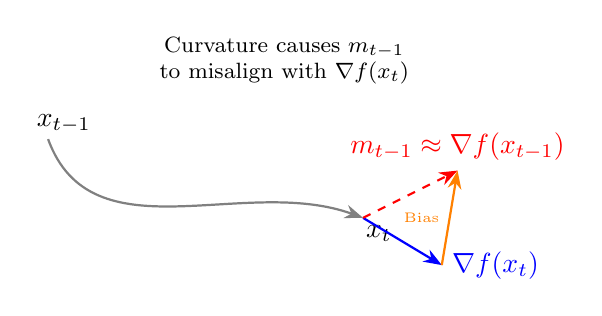
\begin{tikzpicture}[scale=2, >=Stealth]
        % Curved Landscape trajectory
        \draw[thick, gray, ->] (0,1) to[out=-70, in=160] (2,0.5);
        \node at (0.1, 1.1) {$x_{t-1}$};
        \node at (2.1, 0.4) {$x_{t}$};
        
        % Gradient at x_t
        \draw[->, thick, blue] (2,0.5) -- (2.5, 0.2) node[right] {$\nabla f(x_t)$};
        
        % Momentum from previous (Gradient at x_{t-1} transported)
        \draw[->, thick, dashed, red] (2,0.5) -- (2.6, 0.8) node[above] {$m_{t-1} \approx \nabla f(x_{t-1})$};
        
        % Bias Vector
        \draw[->, thick, orange] (2.5, 0.2) -- (2.6, 0.8) node[midway, left] {\tiny Bias};
        
        \node[align=center, font=\footnotesize] at (1.5, 1.5) {Curvature causes $m_{t-1}$\\ to misalign with $\nabla f(x_t)$};
    \end{tikzpicture}
    \caption{\textbf{Momentum Bias.} The historic momentum $m_{t-1}$ approximates $\nabla f(x_{t-1})$, but the optimizer has moved to $x_t$. The deviation (orange vector) is the bias induced by the Hessian $\nabla^2 f$. To accelerate convergence, this bias must be corrected.}
    \label{fig:bias_diagram}
\end{figure}

\subsection{The Landscape of Bias Correction}
\label{subsec:bias_landscape}

To restore the optimal convergence properties of momentum, we must correct the "lag" in the estimator. Mathematically, this requires constructing a correction term $\delta_t$ that acts as an unbiased estimator of the gradient change along the update path, effectively approximating the integral $\nabla f(x_t) - \nabla f(x_{t-1}) \approx \int \nabla^2 f(x) dx$. While the goal is clear, constructing an estimator that is both computationally efficient and valid under weak assumptions has proven to be a difficult balancing act. Prior works have attempted to construct this estimator, but each approach incurs a prohibitive trade-off (summarized in Table~\ref{tab:comparison}).

The first class of methods, exemplified by STORM or MVR \citep{cutkosky2019storm}, estimates the path integral using the difference of stochastic gradients at the two endpoints: $\delta_t = \nabla f_{\xi}(x_t) - \nabla f_{\xi}(x_{t-1})$. While this method maintains a standard cost of $2(F_c+B_c)$ (two gradients per step), its variance is tightly coupled to the smoothness of the individual sample loss functions. Consequently, these methods strictly require that every individual sample $f_\xi$ be smooth (later relaxed to average smoothness). This assumption is frequently violated in modern deep learning architectures, such as those employing ReLU activations, causing the variance of the estimator to explode and training to diverge.

To address the limitations of difference-based estimators, Second-Order Momentum (SOM) \citep{tran2022better} approximates the integral directly using a local linearization around the previous iterate: $\delta_t = \nabla^2 f_{\xi}(x_{t})(x_t - x_{t-1})$. Like STORM, this maintains the standard $2(F_c+B_c)$ cost by reusing gradients. However, because this is a deterministic approximation of the integral using a fixed point, the approximation error is bounded only if the Hessian does not change rapidly. Thus, the classic SOM strictly requires \textbf{both} the gradient and the Hessian to be globally Lipschitz continuous (i.e., bounded second and third derivatives). These are strong, global assumptions that are difficult to verify and often do not hold in practice.

More recent variants, often referred to as SOM-Unif, attempt to relax these smoothness requirements by applying the Mean Value Theorem stochastically. This technique was originally introduced for Frank-Wolfe by \citet{zhang2020one}, later adapted to Reinforcement Learning by \citet{salehkaleybar2022momentum} and recently used for general unconstrained optimization \citep{sadiev2025second, khirirat2025better}. This approach samples a uniform midpoint $\hat{x}$ between $x_{t-1}$ and $x_t$ to evaluate the Hessian term $\delta_t = \nabla^2 f_\xi(\hat{x})(x_t - x_{t-1})$. This provides an unbiased estimator requiring only expected smoothness ($C^2$). However, this theoretical robustness comes at a steep computational price. Since the evaluation point $\hat{x}$ is distinct from the gradient query points ($x_t, x_{t-1}$), the method requires a dedicated forward and backward pass just for the Hessian-Vector Product. This raises the cost to $3(F_c+B_c)$ per iteration, effectively negating much of the wall-clock speedup gained from acceleration.

\begin{table}[ht]
\centering
\small
\setlength{\tabcolsep}{4pt}
\caption{\textbf{Comparison of Momentum Correction Strategies.} Existing methods like STORM \cite{cutkosky2019storm} and Classic SOM \cite{tran2022better} either require strong assumptions (smoothness of individual samples $f_\xi$, Lipschitz Hessian) or, like SOM-Unif \cite{zhang2020one, salehkaleybar2022momentum}, incur higher computational costs due to auxiliary queries. RanSOM is the only method that achieves acceleration with minimal assumptions and standard cost. ($\Delta x_t = x_t - x_{t-1}$; $F_c$=Forward pass, $B_c$=Backward pass; Exp.=Expected, Lip.=Lipschitz; Rates shown assume Bounded Variance).}
\label{tab:comparison}
\begin{tabular}{@{}llclc@{}}
\toprule
\textbf{Method} & \textbf{Estimator $\delta_t$} & \textbf{Smoothness Assumption} & \textbf{Cost} & \textbf{Rate} \\
\midrule
\textbf{STORM} & $\nabla f_\xi(x_t) - \nabla f_\xi(x_{t-1})$ & Average & $2(F_c+B_c)$ & $T^{-1/3}$ \\
\textbf{SOM (Classic)} & $\nabla^2 f_\xi(x_{t}) \Delta x_t$ & Exp. + Lip. $\nabla^2 f$ & $2(F_c+B_c)$ & $T^{-1/3}$ \\
\textbf{SOM-Unif} & $\nabla^2 f_\xi(\hat{x}) \Delta x_t$ & Expected & $\mathbf{3(F_c+B_c)}$ & $T^{-1/3}$ \\
\midrule
\textbf{RanSOM (Ours)} & $\nabla^2 f_\xi(x_t) \Delta x_t$ & \textbf{Expected} & $\mathbf{2(F_c+B_c)}$ & $\mathbf{T^{-1/3}}$ \\
\bottomrule
\end{tabular}
\end{table}

\subsection{Our Contribution: RanSOM}
We propose a solution that eliminates both the additional assumptions and the computational overhead of prior corrections. We introduce \textbf{Randomized Second-Order Momentum (RanSOM)}, a framework based on a novel paradigm: \textit{Randomized Step Sizes}.

Instead of a fixed step $\eta_t$, we treat the step size $s_t$ as a random variable:
\begin{equation*}
    x_{t+1} = x_t + s_t d_t, \quad \text{where } \mathbb{E}[s_t] = \eta_t.
\end{equation*}
By randomizing the step (e.g., via Exponential or Beta distributions), we utilize identities analogous to \textbf{Stein's Lemma} to perform "statistical integration" of the Hessian. This yields an exact, unbiased estimator of the curvature bias using a single Hessian-Vector Product (HVP) at the \textit{next} iterate $x_{t+1}$.

Our approach offers three distinct advantages:

\begin{enumerate}
    \item \textbf{Universal Geometric Framework:} We couple our randomized correction with \textit{Linear Minimization Oracle (LMO)} updates. This allows RanSOM to naturally generalize modern "normalized" optimizers:
    \begin{itemize}
        \item With an $L_2$-ball LMO, we recover \textit{Normalized SGD}.
        \item With an $L_\infty$-ball LMO, we recover \textit{SignSGD}.
        \item With spectral constraints, we can extend to \textit{Muon}-style updates.
    \end{itemize}
    
    \item \textbf{Optimal Rate and Generalized Robustness:} We provide a rigorous convergence analysis proving that RanSOM achieves the optimal $\mathcal{O}(\epsilon^{-3})$ sample complexity under standard bounded variance assumptions. Furthermore, we extend our analysis to challenging non-standard settings, demonstrating that RanSOM converges robustly even under \textit{generalized $(L_0, L_1)$-smoothness} and \textit{heavy-tailed gradient noise} ($p \in (1, 2]$), without requiring the Hessian to be Lipschitz continuous.
    \item \textbf{No Auxiliary Query Overhead:} Unlike variance-reduced methods such as SOM-Unif which require sampling auxiliary "look-ahead" points, RanSOM evaluates the Hessian-Vector Product at $x_{t+1}$—the same point required for the subsequent gradient step. While this incurs the computational cost of a second backpropagation pass (similar to STORM), it avoids the additional data loading and forward pass overhead associated with auxiliary queries.
\end{enumerate}

\section{Related Work}
\label{sec:related_work}

\textbf{Bias in Stochastic Momentum.} 
Standard momentum (SGDM) \cite{polyak1964, sutskever2013importance} suffers from a curvature-induced bias in non-convex settings \cite{yuan2016convergence}. This prevents optimal convergence unless the momentum parameter $\beta$ decays rapidly, which often causes training instability.

\textbf{Variance Reduction and Acceleration.} 
Recursive variance reduction achieves the optimal $\mathcal{O}(\epsilon^{-3})$ sample complexity. STORM \cite{cutkosky2019storm} eliminated SPIDER's \cite{fang2018spider} full-gradient requirement using a recursive estimator. While  recent works like \citet{khirirat2025better} showed that STORM converges under ``average smoothness'' rather than strictly smooth individual losses, this remains a strictly stronger assumption than classical expected smoothness. Crucially, while average smoothness bounds the expected squared difference of stochastic gradients (which still severely restricts non-smooth realizations like ReLUs), expected smoothness only requires the macroscopic objective $f(x) = \mathbb{E}[f_\xi(x)]$ to be smooth. This allows RanSOM to naturally handle non-smooth individual losses where prior methods fail.

\textbf{Geometric Optimization \& Second-Order Correction.}
Adapting momentum to non-Euclidean geometries via Linear Minimization Oracles (LMOs) \cite{jordan2024muon, pethick2025training, kovalev2025non} typically yields a slower $\mathcal{O}(\epsilon^{-4})$ rate. Second-Order Momentum (SOM) corrects bias using Hessian information \cite{tran2022better, khirirat2025better} to recover the $\mathcal{O}(\epsilon^{-3})$ rate, but introduces a strict trade-off: it either requires Hessian Lipschitz continuity, or it demands an auxiliary "lookahead" evaluation point (SOM-Unif) that doubles computational costs \cite{zhang2020one, salehkaleybar2022momentum, sadiev2025second, khirirat2025better}. RanSOM resolves this dilemma, integrating sampling directly into the update step via Stein's Identity to achieve the optimal rate without auxiliary points or Lipschitz Hessian assumptions.

\textbf{Robustness to Heavy Tails and Relaxed Smoothness.} 
Standard methods struggle with heavy-tailed gradient noise ($p \in (1, 2]$) and non-uniform smoothness. \citet{hubler2025gradient} showed gradient normalization achieves optimal convergence under heavy tails, while \citet{chen2023generalized} introduced $(L_0, L_1)$-smoothness for modern architectures like Transformers. RanSOM generalizes both: our LMO update inherently normalizes heavy tails, and our integration-based bias correction holds under generalized $(L_0, L_1)$-smoothness.

\textbf{Connections to Stein's Identity and Second-Order Momentum.} 
While \citet{zhang2024random} pioneered the exponential identity to smooth non-smooth objectives, we fundamentally repurpose it to estimate and bound momentum bias in constrained optimization under $(L_0, L_1)$-smoothness. We additionally introduce a novel Beta identity specifically tailored for unconstrained settings. 

Finally, our ``second-order momentum'' integrates Hessian-vector products into the estimator to track update-path curvature without forming full matrices. This is distinct from ``momentum for second-order optimization'' (e.g., stochastic cubic Newton \cite{chayti2024improving}), which solves complex cubic subproblems to attain faster deterministic rates under stronger theoretical assumptions, though this approach achieves a weaker stochastic rate.

\section{Method: The RanSOM Framework}
\label{sec:method}

Standard momentum fails in non-convex settings because the accumulated gradient vector $m_t$ becomes stale as the optimizer traverses curved landscapes. To correct this, we need to estimate the integral of the Hessian along the update path.
The core intuition of RanSOM is that \textit{randomization acts as a probe for curvature}. By treating the step size not as a fixed hyperparameter but as a random variable drawn from a specific distribution, we can exploit integration-by-parts identities (Stein's Lemma) to relate the finite difference of gradients (the bias) to a single point-derivative (the Hessian-Vector Product).

\subsection{Randomized Integration by Parts}
We define the ``gradient along the path'' function $g(s) = \nabla f(x_t + s d_t)$, where $d_t$ is the update direction. The bias we wish to estimate is the expected change in gradients:
$$ \Delta = \mathbb{E}[g(s) - g(0)] = \mathbb{E}[\nabla f(x_{t+1}) - \nabla f(x_t)]. $$
Directly computing this expectation typically requires two evaluations ($x_t$ and $x_{t+1}$). However, using Stein-type identities, we can express this difference using only the derivative $g'(s) = \nabla^2 f(x_t + s d_t) d_t$ evaluated at the \textit{random} endpoint $s$.

\begin{lemma}[Stein-Type Identities for Optimization]
\label{lemma:stein}
Let $g: \mathbb{R} \to \mathbb{R}^d$ be a differentiable function with
\emph{integrable derivative} (i.e. $\int_0^\infty \|g'(z)\|_2\, dz <
\infty$).
\begin{enumerate}
    \item \textbf{Exponential Identity (Unconstrained):} If
    $s \sim \mathrm{Exp}(\lambda)$, then
    \begin{equation}
        \mathbb{E}[g(s) - g(0)] = \frac{1}{\lambda} \mathbb{E}[g'(s)].
    \end{equation}
    This implies that scaling the Hessian-Vector Product at the
    destination $x_{t+1}$ by $\eta_t = 1/\lambda$ yields an unbiased
    estimator of the gradient difference.
 
    \item \textbf{Beta Identity (Constrained):} If
    $s \sim \mathrm{Beta}(1, K)$, then
    \begin{equation}
        \mathbb{E}[g(s) - g(0)]
        = \mathbb{E}\!\left[\tfrac{1-s}{K}\, g'(s)\right].
    \end{equation}
    The Hessian-Vector Product is re-weighted by $(1-s)/K$ to account
    for the compact support of the Beta distribution.
\end{enumerate}
\end{lemma}
 
\textit{Proof sketch.} Both identities follow from the integration-by-parts
formula
\[
    \mathbb{E}[g(s)-g(0)] = \int_0^\infty g'(z)\,(1 - F(z))\, dz,
\]
where $F$ is the CDF of $s$. For $s \sim \mathrm{Exp}(\lambda)$, the
survival function $1-F(z) = e^{-\lambda z}$ is proportional to the PDF,
yielding the scalar factor $1/\lambda$. For $s \sim \mathrm{Beta}(1, K)$,
the survival function $(1-z)^K$ gives the weight $(1-z)/K$ times the
PDF. See Appendix~\ref{app:stein} for the full proof.


\subsection{Joint Efficient Computation via Automatic Differentiation}
A critical theoretical advantage of RanSOM translates directly into practical efficiency. The correction term requires evaluating the Hessian-Vector Product (HVP) $h_{t+1} = \nabla^2 f(x_{t+1}) d_t$ at the \textit{next} iterate $x_{t+1}$.
In modern Automatic Differentiation (AD) frameworks (e.g., PyTorch, JAX), this operation does \textbf{not} require materializing the full Hessian. Instead, it is computed via Pearlmutter's trick:
\begin{equation}
    h_{t+1} = \nabla_{x} (\langle \nabla f(x_{t+1}), \text{stop\_grad}(d_t) \rangle).
\end{equation}
Crucially, this computation shares the forward pass and the backward graph with the standard gradient computation. By computing the gradient $g_{t+1} = \nabla f(x_{t+1})$ and the HVP $h_{t+1}$ in a single combined backward pass, the total cost is roughly $2\times$ that of a standard forward pass—comparable to standard SGD and significantly cheaper than methods requiring auxiliary point evaluations (which cost $3\times$ or more).

\subsection{Algorithm~\ref{alg:expsom}: RanSOM-E (Unconstrained / Normalized)}
For unconstrained optimization on $\mathbb{R}^d$, we employ \textit{the Exponential Identity}. To handle potential heavy-tailed noise and adapt to the geometry, we determine the update direction using a Linear Minimization Oracle (LMO) over a norm ball $\mathcal{B}_\rho = \{v : \|v\| \le \rho\}$ (see Algorithm~\ref{alg:expsom}). This framework naturally unifies several modern optimization paradigms:

\begin{itemize}
    \item \textbf{Euclidean Case ($L_2$):} The LMO yields $d_t = -\rho \frac{m_t}{\|m_t\|_2}$. This recovers \textbf{Normalized SGD}, connecting our method to robust techniques but with added acceleration.
    \item \textbf{Coordinate-Wise Geometry ($L_\infty$):} The LMO yields $d_t = -\rho \cdot \text{sign}(m_t)$. This recovers \textbf{SignSGD}~\cite{bernstein2018signsgd}, known for its communication efficiency and robustness to magnitude variance.
    \item \textbf{Spectral Geometry (Schatten Norms):} For matrix parameters (e.g., in Transformers), the LMO can enforce spectral constraints. This recovers \textbf{Muon}-style updates~\cite{jordan2024muon}, where $d_t$ is computed via Newton-Schulz iterations to orthogonalize the update.
\end{itemize}

\begin{figure*}[t]
    \centering
    % --- Left Column: RanSOM-E ---
    \begin{minipage}{0.48\textwidth}
        \begin{algorithm}[H]
            \caption{RanSOM-E: Exponential-Distributed Second-Order Momentum}
            \label{alg:expsom}
            \begin{algorithmic}[1]
                \STATE {\bfseries Input:} Initial $x_0$, rate $\eta_t$, mom. $\beta$, radius $\rho$, batches $B_{init},B$
                \STATE Initialize $m_0 = \frac{1}{B_{init}} \sum_{\xi \in \mathcal{B}_0} \nabla f_{\xi}(x_0)$
                \FOR{$t=0$ {\bfseries to} $T-1$}
                \STATE \textit{// 1. Geometric Update Direction (LMO)}
                \STATE Solve $d_t = \argmin_{v : \|v\| \le \rho} \langle m_t, v \rangle$
                \STATE \quad $\triangleright$ \textbf{Norm. SGD:} $d_t \leftarrow -\rho \cdot m_t / \|m_t\|_2$
                \STATE \quad $\triangleright$ \textbf{SignSGD:} $d_t \leftarrow -\rho \cdot \text{sign}(m_t)$
                \STATE \quad $\triangleright$ \textbf{Muon:} $d_t \leftarrow -\rho \cdot \text{NewtonSchulz}(m_t)$
                
                \STATE \textit{// 2. Randomized Step (Stein's Trick)}
                \STATE Sample $s_t \sim \mathrm{Exp}(1/\eta_t)$ 
                \STATE Update: $x_{t+1} = x_t + s_t d_t$
                
                \STATE \textit{// 3. Joint Computation}
                \STATE Sample batch $\mathcal{B}_{t+1}$
                \STATE Compute $(g_{t+1}, h_{t+1})$ via sim. backprop:
                \STATE \quad $g_{t+1} = \frac{1}{B} \sum_{\xi \in \mathcal{B}_{t+1}} \nabla f_{\xi}(x_{t+1})$
                \STATE \quad $h_{t+1} = \frac{1}{B} \sum_{\xi \in \mathcal{B}_{t+1}} \nabla^2 f_{\xi}(x_{t+1}) d_t$
                
                \STATE \textit{// 4. Bias Correction}
                \STATE Estimate Bias: $\delta_{t+1} = \eta_t \cdot h_{t+1}$ 
                \STATE Update $m_{t+1} = (1-\beta)(m_t + \delta_{t+1}) + \beta g_{t+1}$
                \ENDFOR
            \end{algorithmic}
        \end{algorithm}
    \end{minipage}
    \hfill % Adds spacing between the two minipages
    % --- Right Column: RanSOM-B ---
    \begin{minipage}{0.48\textwidth}
        \begin{algorithm}[H]
            \caption{RanSOM-B: Beta-Distributed Second-Order Momentum}
            \label{alg:betasom}
            \begin{algorithmic}[1]
                \STATE {\bfseries Input:} $x_0 \in \mathcal{C}$, rate $\eta_t \in (0, 1)$, mom. $\beta$, batches $B_{init},B$
                \STATE Initialize $m_0 = \frac{1}{B_{init}} \sum_{\xi \in \mathcal{B}_0} \nabla f_{\xi}(x_0)$
                \FOR{$t=0$ {\bfseries to} $T-1$}
                \STATE \textit{// 1. Frank-Wolfe Direction}
                \STATE Solve LMO: $v_t = \argmin_{v \in \mathcal{C}} \langle m_t, v \rangle$
                \STATE Set direction: $d_t = v_t - x_t$
                
                \STATE \textit{// 2. Randomized Feasible Step}
                \STATE Set parameter $K_t = \frac{1}{\eta_t} - 1$
                \STATE Sample $s_t \sim \mathrm{Beta}(1, K_t)$ 
                \STATE Update: $x_{t+1} = x_t + s_t d_t$ 
                
                \STATE \textit{// 3. Joint Computation}
                \STATE Sample batch $\mathcal{B}_{t+1}$ and compute $(g_{t+1}, h_{t+1})$ at $x_{t+1}$
                \vspace{2.25em} % Adjust to align lines with left algorithm
                
                \STATE \textit{// 4. Weighted Bias Correction}
                \STATE Calculate Stein Weight: $w_t = \frac{1-s_t}{K_t}$
                \STATE Estimate Bias: $\delta_{t+1} = w_t \cdot h_{t+1}$
                \STATE Update $m_{t+1} = (1-\beta)(m_t + \delta_{t+1}) + \beta g_{t+1}$
                \ENDFOR
                \vspace{0.35em} % Small buffer for visual alignment
            \end{algorithmic}
        \end{algorithm}
    \end{minipage}
\end{figure*}


\subsection{Algorithm~\ref{alg:betasom}: RanSOM-B (Constrained)}
For constrained optimization over a convex set $\mathcal{C}$, using an Exponential step size is invalid because $x_{t+1}$ might leave the domain. Instead, we use the \textit{Beta Identity}. We draw steps from a Beta distribution supported on $[0, 1]$, ensuring that the convex combination $x_{t+1} = (1-s_t)x_t + s_t v_t$ remains strictly feasible (see Algorithm~\ref{alg:betasom}).


\section{Theoretical Analysis}
\label{sec:theory}

In this section, we establish the convergence of RanSOM for non-convex optimization. Our analysis highlights three key theoretical advantages of the proposed framework:

\begin{enumerate}
    \item \textbf{Minimal Assumptions:} Unlike recursive variance reduction methods such as STORM~\cite{cutkosky2019storm} or SPIDER~\cite{fang2018spider}, we do \textbf{not} require the individual stochastic functions $f_\xi(x)$ to be smooth (almost surely), nor do we assume bounded variance. We handle heavy-tailed noise directly, similar to recent robust techniques~\cite{liu2023nonconvex, hubler2025gradient}. Furthermore, unlike prior second-order methods (e.g., \cite{tran2022better, khirirat2025better}), we do \textbf{not} require the Hessian to be Lipschitz continuous.
    
    \item \textbf{No Overhead:} Our correction term uses a Hessian-vector product at $x_{t+1}$, which is the exact point required for the gradient evaluation in the subsequent step. This avoids the need for "look-ahead" points or double-evaluations common in other variance-reduced estimators like SOM-Unif~\cite{salehkaleybar2022momentum, zhang2020one}.
    
    \item \textbf{Clipping-Free:} We achieve optimal convergence rates without the need for gradient clipping. By identifying the appropriate batch size and step size scaling, RanSOM naturally handles heavy-tailed noise, generalizing the normalization benefits observed in first-order methods~\cite{hubler2025gradient}.
\end{enumerate}

\subsection{Preliminaries \& Notation}

We consider optimization over a finite-dimensional real vector space $\mathcal{E} = \R^d$ equipped with a general norm $\|\cdot\|$.
\begin{itemize}
    \item \textbf{Primal Norm:} For $x \in \mathcal{E}$, we denote the norm by $\|x\|$.
    \item \textbf{Dual Norm:} The space of gradients is the dual space $\mathcal{E}^*$. For $g \in \mathcal{E}^*$, the dual norm is defined as $\|g\|_* := \sup_{\|x\| \le 1} \langle g, x \rangle$.
    \item \textbf{Operator Norm:} The Hessian $\nabla^2 f(x)$ is a linear operator mapping $\mathcal{E} \to \mathcal{E}^*$. We define the induced operator norm as:
    \begin{equation*}
        \|\nabla^2 f(x)\|_{op} := \sup_{\|u\| \le 1} \|\nabla^2 f(x) u\|_* = \sup_{\|u\| \le 1, \|v\| \le 1} \langle \nabla^2 f(x) u, v \rangle.
    \end{equation*}
\end{itemize}

\subsection{Assumptions}

We analyze our method under generalized assumptions capturing modern deep learning dynamics.

\begin{assumption}[Well--Defined Problem]
\label{ass:well_defined}
$f : \mathcal{E} \to \mathbb{R}$ is bounded below by $f_* > -\infty$; let
$\Delta_0 \triangleq f(x_0) - f_*$.
\end{assumption}

\begin{assumption}[Pointwise $(L_0, L_1)$--Smoothness]
\label{ass:geometric_smoothness}
$f$ is twice continuously differentiable and there exist constants
$L_0, L_1 \geq 0$ such that
\begin{equation}
  \|\nabla^2 f(x)\|_{\mathrm{op}}
  \;\leq\; L_0 + L_1 \|\nabla f(x)\|_*
  \qquad \text{for every } x \in \mathcal{E}.
\end{equation}
\end{assumption}

\begin{assumption}[Norm Compatibility]
\label{ass:norm_compatibility}
There exists $\kappa \geq 1$ such that $\|u\|_* \leq \kappa \|u\|_2$ and
$\|u\|_2 \leq \kappa \|u\|_*$ for every $u \in \mathcal{E}^* \cup
\mathcal{E}$.
\end{assumption}

\begin{assumption}[Affine Heavy--Tailed Noise]
\label{ass:noise}
The stochastic gradient $g(x) = \nabla f_\xi(x)$ and the Hessian--vector
product oracle $H(x)w = \nabla^2 f_\xi(x) w$ are unbiased, and there
exist constants $\sigma_g, \alpha_g, \sigma_h, \alpha_h \geq 0$ and
exponents $p, q \in (1, 2]$ such that, for every $x \in \mathcal{E}$ and
every deterministic $w \in \mathcal{E}$ independent of the oracle noise
$\xi$,
\begin{align}
  \mathbb{E}_\xi\bigl[\|g(x) - \nabla f(x)\|_2^p \,\big|\, x\bigr]
    &\leq \sigma_g^p + \alpha_g^p \|\nabla f(x)\|_*^p, \\
  \mathbb{E}_\xi\bigl[\|(H(x) - \nabla^2 f(x))w\|_2^q \,\big|\, x, w\bigr]
    &\leq \bigl(\sigma_h^q + \alpha_h^q \|\nabla f(x)\|_*^q\bigr) \|w\|^q.
\end{align}
\end{assumption}

\textbf{Discussion on Assumptions.} Our framework relaxes classical restrictions to capture state-of-the-art non-convex optimization dynamics. Assumption~\ref{ass:geometric_smoothness} models the "exploding gradient" problem prevalent in Transformers \cite{zhang2019gradient}. Furthermore, Assumption~\ref{ass:noise} unifies affine variance growth \cite{bottou2018optimization} with heavy-tailed noise ($p, q < 2$) \cite{simsekli2019tail}, generalizing standard robust momentum methods that strictly assume bounded variance or specific tail indices \cite{cutkosky2019storm, gorbunov2020stochastic}.

\textbf{Simplified Setting.} For clarity, main-text theorems are presented under a standard simplified setting: $L_1 = 0$ (globally bounded Hessian), $\alpha_g = \alpha_h = 0$ (no affine noise growth), and batch size $B=1$ (the initial batch $B_{\mathrm{init}}$ is still chosen large enough to suppress initialization error). General convergence results recovering arbitrary $L_1, \alpha_g, \alpha_h \ge 0$ and $B \ge 1$ are fully detailed in Appendix~\ref{app:theory}.
\subsection{Unconstrained Optimization (RanSOM-E)}

%We analyze RanSOM-E in the unconstrained setting under the standard assumption of bounded noise moments ($\alpha_g = \bar{\alpha}_h = 0$) and relaxed third-order smoothness ($L_1 \approx 0$). 
The convergence analysis relies on bounding the momentum estimation error $e_t = m_t - \nabla f(x_t)$ and coupling it with a descent inequality derived from the Exponential step distribution.

\begin{lemma}[Descent Inequality]
\label{lemma:main_descent}
Let $C_s = \mathbb{E}[s_t^2]/\eta_t^2 = 2$ denote the second moment
constant of $s_t \sim \mathrm{Exp}(1/\eta_t)$, and let $\kappa$ be the
norm compatibility constant of Assumption~\ref{ass:norm_compatibility}.
For any step size $\eta_t \le 1/(\rho L_0)$, the RanSOM-E update
satisfies
\begin{equation}
\label{eq:main_descent}
    \mathbb{E}[f(x_{t+1})] - f(x_t)
    \le -\frac{\rho \eta_t}{2}\,\mathbb{E}[\|\nabla f(x_t)\|_*]
      + 2\rho\kappa\eta_t\,\mathbb{E}[\|e_t\|_2]
      + \frac{C_s \rho^2 L_0}{2}\,\eta_t^2,
\end{equation}
where $e_t = m_t - \nabla f(x_t)$ is the momentum error.
\end{lemma}
 
\noindent The proof combines a Taylor expansion with $L_0$-smoothness
and the LMO optimality of $d_t$; see Appendix~\ref{app:descent-e} for
details (which also covers the general $(L_0, L_1)$ case).


\noindent The critical challenge is bounding the accumulated error
$\mathbb{E}[\|e_t\|_2]$. By the von Bahr-Esseen inequality for
martingale difference sequences, we obtain a bound depending explicitly
on the noise indices $p, q$.
 
\begin{lemma}[Momentum Error Bound]
\label{lemma:main_error}
Under the simplified setting, for any $\beta \in (0, 1/2]$ and $B = 1$,
the averaged momentum error satisfies
\begin{equation}
\label{eq:main_error}
    \frac{1}{T}\sum_{t=0}^{T-1}\mathbb{E}[\|e_t\|_2]
    \le \underbrace{\mathcal{O}\!\left(\frac{\sigma_g}{\beta T\, B_{\mathrm{init}}^{1-1/p}}\right)}_{\text{Initialization}}
    + \underbrace{\mathcal{O}\!\left(\beta^{1-1/p}\,\sigma_g\right)}_{\text{Gradient Noise}}
    + \underbrace{\mathcal{O}\!\left(\eta\,\beta^{-1/q}\,\bar\sigma_h\right)}_{\text{Hessian Bias}},
\end{equation}
where $\bar\sigma_h = \rho(\sigma_h + \kappa L_0)$ is the effective
Hessian-noise constant.
\end{lemma}
 
\noindent Note the asymmetric scaling: the gradient noise contribution
shrinks with $\beta^{1-1/p}$ (smaller momentum helps average out
high-variance gradients) while the Hessian bias \emph{grows} with
$\beta^{-1/q}$ (smaller momentum makes the correction more impactful).
The optimal $\beta$ balances these two opposing effects.


\noindent Combining Lemmas~\ref{lemma:main_descent}
and~\ref{lemma:main_error} and optimizing $\eta$ and $\beta$ yields our
main theorem.
 
\begin{theorem}[Convergence of RanSOM-E]
\label{thm:expsom_convergence}
Let $A = \frac{p-1}{p}$ and $K = \frac{1}{q}$. Under the simplified
setting, and with the optimal choice
\begin{equation}
    \eta \asymp T^{-\frac{q(p-1)+p}{2q(p-1)+p}},
    \qquad
    \beta \asymp T^{-\frac{pq}{2q(p-1)+p}},
\end{equation}
and with $B_{\mathrm{init}}$ chosen large enough that the
initialization term is dominated by the main rate, RanSOM-E converges
to a stationary point at the rate
\begin{equation}
\label{eq:expsom_rate}
    \frac{1}{T}\sum_{t=0}^{T-1}\mathbb{E}[\|\nabla f(x_t)\|_*]
    \le 
    \mathcal{O}\!\left(\underbrace{
        (\Delta_0\bar\sigma_h)^{\tfrac{A}{2A+K}}\,
        \sigma_g^{\tfrac{K}{2A+K}}\;
        T^{-\tfrac{q(p-1)}{2q(p-1)+p}}
    }_{\text{Main Variance Rate}}
    + \underbrace{\sqrt{\Delta_0 L_0}\, T^{-1/2}}_{\text{Smoothness Rate}}
    + \underbrace{\Delta_0 L_0\, T^{-1}}_{\text{Geometric Limit Rate}}\right).
\end{equation}
\end{theorem}
 
\textbf{Optimal Rate ($p = q = 2$).}
In the standard setting with finite variance ($A = K = 1/2$), the main
rate specializes to
\[
    \mathcal{O}\!\left((\Delta_0\,\sigma_g\,\bar\sigma_h)^{1/3}\,T^{-1/3}\right),
\]
matching the optimal rate for non-convex stochastic optimization
\cite{cutkosky2019storm, arjevani2023lower}. The associated optimal
momentum is $\beta \asymp T^{-2/3}$, consistent with the classical
STORM scaling.
 
\textbf{Optimality ($p = q$).}
When $p = q$, the main rate simplifies to $\mathcal{O}(T^{-(p-1)/(2p-1)})$,
matching the optimal sample complexity established by
\citet{sadiev2025second}. RanSOM achieves this through its intrinsic
LMO-based normalization, without explicit gradient or Hessian clipping.
 


\subsection{Constrained Optimization (RanSOM-B)}

For constrained problems, we minimize $f(x)$ over a compact convex set $\mathcal{C}$ with diameter $D \triangleq \sup_{x,y \in \mathcal{C}} \|x-y\|$. We use the Frank-Wolfe gap $\mathcal{G}(x) = \max_{v \in \mathcal{C}} \langle \nabla f(x), x-v \rangle$ as the convergence criterion.

\begin{lemma}[Constrained Descent Inequality]
\label{lemma:constrained_descent}
Let $s_t \sim \mathrm{Beta}(1, K_t)$ with mean $\eta_t = 1/(1 + K_t)$.
The second moment satisfies $\mathbb{E}[s_t^2] = C_s\,\eta_t^2$ with
$C_s = 2(1+K_t)/(2+K_t) \le 2$. Under the simplified setting ($L_1 =
0$, so $L_0$-smoothness is global on $\mathcal{C}$), the RanSOM-B
update satisfies
\begin{equation}
\label{eq:constrained_descent}
    \mathbb{E}[f(x_{t+1})] - f(x_t)
    \le -\eta_t\,\mathbb{E}[\mathcal{G}(x_t)]
      + 2D\eta_t\,\mathbb{E}[\|e_t\|_2]
      + \frac{C_s L_0 D^2}{2}\,\eta_t^2.
\end{equation}
%where $\mathcal{G}(x) = \max_{v \in \mathcal{C}}\langle\nabla f(x), x-v\rangle$ is the Frank-Wolfe gap and $D = \sup_{x, y \in \mathcal{C}}\|x-y\|$ is the diameter.
\end{lemma}


\begin{theorem}[Convergence of RanSOM-B]
\label{thm:betasom_convergence}
Under the same simplified setting as Theorem~\ref{thm:expsom_convergence},
and using the Beta-distributed step size, RanSOM-B satisfies
\begin{equation}
\label{eq:betasom_rate}
    \frac{1}{T}\sum_{t=0}^{T-1}\mathbb{E}[\mathcal{G}(x_t)]
    \le
    \mathcal{O}\!\left(\underbrace{
        (\Delta_0\bar\sigma_h)^{\tfrac{A}{2A+K}}\,
        (D\sigma_g)^{\tfrac{K}{2A+K}}\,
        T^{-\tfrac{q(p-1)}{2q(p-1)+p}}
    }_{\text{Main Variance Rate}}
    + \underbrace{D\sqrt{\Delta_0 L_0}\,T^{-1/2}}_{\text{Smoothness Rate}}
    + \underbrace{\Delta_0\,T^{-1}}_{\text{Geometric Limit Rate}}\right),
\end{equation}
where $\bar\sigma_h = D(\sigma_h + L_0)$ is the effective Hessian-noise
constant on the compact set $\mathcal{C}$.
 
For the standard case $p = q = 2$, the main rate recovers the optimal
$\mathcal{O}(T^{-1/3})$ scaling for projection-free methods, with
constant $\mathcal{O}((\Delta_0 \cdot D\sigma_g \cdot \bar\sigma_h)^{1/3})$.
\end{theorem}


\section{Numerical Experiments}

We evaluate the RanSOM framework on three non-convex tasks: (1) binary classification (SPLICE), (2) sequence classification (MNIST1D), and (3) constrained matrix completion (MovieLens). Results for SPLICE and MovieLens are provided in Appendix \ref{sec:AppExp}. This section focuses on MNIST1D to compare our unconstrained (RanSOM-E) variant against state-of-the-art baselines.

\textbf{MNIST1D Results.} We utilize the MNIST1D benchmark \cite{mnist1d} to test curvature correction in deep, non-convex landscapes. As shown in Figure \ref{fig:mnist1d_results} and Table \ref{tab:mnist1d_results}, \textbf{RanSOM-E (Muon)} outperforms all baselines, achieving a peak accuracy of $\mathbf{91.90\%}$. While STORM exhibits significant instability ($88.83\% \pm 1.38$), RanSOM-E maintains high precision and low variance ($\pm 0.36$), empirically validating the robustness of our randomized bias correction.

\begin{figure}[h]
    \centering    \includegraphics[width=0.85\linewidth]{MNIST1DRanSOMEXP2-1.pdf}
    \caption{Training Loss and Test Accuracy on MNIST1D. RanSOM-E variants demonstrate superior convergence over first-order and classic second-order baselines.}
    \label{fig:mnist1d_results}
\end{figure}

\begin{table}[h]
    \centering
    \small
    \caption{Test Accuracy on MNIST1D (Mean $\pm$ Std, 3 runs)}
    \label{tab:mnist1d_results}
    \begin{tabular}{lc}
        \toprule
        \textbf{Optimizer} & \textbf{Test Accuracy (\%)} \\
        \midrule
        STORM           & $88.83 \pm 1.38$ \\
        SOM-Classic     & $86.87 \pm 0.75$ \\
        Muon            & $91.50 \pm 0.90$ \\
        RanSOM-E (Norm) & $90.97 \pm 0.84$ \\
        \textbf{RanSOM-E (Muon)} & $\mathbf{91.90 \pm 0.36}$ \\
        \bottomrule
    \end{tabular}
\end{table}
\section{Discussion and Conclusion}
\label{sec:discussion}

Standard momentum methods often suffer from curvature-induced bias in non-convex landscapes. To address this, we introduced \textbf{RanSOM}, a framework that utilizes randomized integration and Stein-type identities to construct an unbiased gradient estimator via a single Hessian-vector product. RanSOM recovers the optimal $\mathcal{O}(T^{-1/3})$ convergence rate under bounded variance and maintains optimality even with heavy-tailed noise. Critically, it resolves two major limitations of prior second-order corrections: it requires no extra assumptions—avoiding the need for individual/average sample smoothness or Lipschitz Hessians—and incurs no extra cost, matching the query complexity of standard variance reduction methods without auxiliary oracle queries.

\textbf{Empirical Validation.} Experiments on SPLICE and MNIST1D confirm that RanSOM-E offers significantly higher stability than STORM, validating our correction under heavy-tailed noise. In constrained settings, RanSOM-B outperformed SFW baselines on MovieLens, suggesting that Beta-distributed steps effectively navigate complex constraint geometries.

\textbf{Limitations and Future Work.} While theoretically efficient, the required HVP incurs a computational cost roughly double that of SGD. Furthermore, tuning the step-size distribution parameters for heterogeneous landscapes remains a challenge. Future research will explore adaptive distributions and applications within reinforcement learning.

\textbf{Conclusion.} RanSOM provides a unified, assumption-light framework for non-convex optimization. By treating step sizes as random variables, it enables robust second-order bias correction without Lipschitz assumptions on the Hessian or the typical computational overhead of auxiliary sampling.


\bibliography{example_paper}
\bibliographystyle{icml2026}


%%%%%%%%%%%%%%%%%%%%%%%%%%%%%%%%%%%%%%%%%%%%%%%%%%%%%%%%%%%%%%%%%%%%%%%%%%%%%%%
% APPENDIX
%%%%%%%%%%%%%%%%%%%%%%%%%%%%%%%%%%%%%%%%%%%%%%%%%%%%%%%%%%%%%%%%%%%%%%%%%%%%%%%
\newpage
\onecolumn
\appendix

%%%%%%%%%%%%%%%%%%%%%%%%%%%%%%%%%%%%%%%%%%%%%%%%%%%%%%%%%%%%%%%%%%%%%%%%%%%%%

\section{Additional Experiments}\label{sec:AppExp}
\subsection{Non-Convex Classification: Splice Dataset}

\textbf{Setup.} We evaluate performance on the Splice dataset from the LibSVM repository \cite{libsvm}, utilizing a Multi-Layer Perceptron (MLP) architecture ($60 \to 32 \to 16 \to 1$). To introduce challenging non-convexity into the loss landscape, we employ Welsch regularization. The objective function is given by:
\[
\mathcal{L}(w) = \text{BCE}(w) + \lambda \sum_{i} \frac{w_i^2}{1 + w_i^2}
\]
where $\lambda=0.1$. We compare RanSOM-E (using both Normalized and Muon-style updates) against SGD with Momentum (SGDm), classic Second-Order Momentum (SOM), Muon, and STORM.

\textbf{Results.} Figure \ref{fig:splice_results} illustrates the training loss and test accuracy trajectories. RanSOM-E (Muon) demonstrates rapid convergence and superior stability compared to the baselines. As detailed in Table \ref{tab:results}, RanSOM-E (Muon) achieves the highest final test accuracy of $\mathbf{84.90\%} \pm 0.0038$, outperforming the closest competitor (Muon) while maintaining significantly lower variance than STORM.

\begin{figure}[h]
    \centering    \includegraphics[width=1\linewidth]{SpliceExp-2.pdf}
    \caption{Training Loss (left) and Test Accuracy (right) on the Splice dataset with Welsch regularization. RanSOM-E (Muon) shows the fastest convergence and highest final accuracy.}
    \label{fig:splice_results}
\end{figure}
\vspace*{-\baselineskip}
\begin{table}[h]
    \centering
    \caption{Comparison of Final Test Accuracy on SPLICE dataset}
    \label{tab:results}
    \begin{tabular}{lc}
        \toprule
        \textbf{Optimizer} & \textbf{Test Accuracy (\%)} \\
        \midrule
        SGDm & $0.8392 \pm 0.0061$ \\
        SOM & $0.8342 \pm 0.0118$ \\
        Muon & $0.8466 \pm 0.0079$ \\
        STORM & $0.7335 \pm 0.1077$ \\
        RanSOM-E (Norm) & $0.8441 \pm 0.0052$ \\
        RanSOM-E (Muon) & $\mathbf{0.8490 \pm 0.0038}$ \\
        \bottomrule
    \end{tabular}
\end{table}

\subsection{Constrained Matrix Completion: Nano MovieLens}

\textbf{Setup.} To evaluate the constrained variant RanSOM-B, we perform matrix completion on the "Nano" MovieLens dataset (a subset of MovieLens 100K \cite{movielens} consisting of the top 100 users and 200 movies). The problem is formulated as minimizing the reconstruction error (RMSE) under a Nuclear Norm ball constraint, a classic non-convex constrained problem. We compare RanSOM-B against Stochastic Frank-Wolfe with Polyak Momentum (SFW-Polyak) and Stochastic Frank-Wolfe with Classic SOM (SFW-SOM).

\textbf{Results.} Figure \ref{fig:movielens_results} displays the RMSE trajectories over 50 epochs.
\begin{itemize}[topsep=0pt]
    \item \textbf{Performance:} RanSOM-B achieves the lowest final average RMSE, demonstrating that the randomized Beta-distributed steps effectively navigate the constrained geometry better than deterministic step sizes.
    \item \textbf{Stability:} While RanSOM-B exhibits marginally higher variance in the earliest epochs (attributed to the exploration inherent in the randomized step size), it quickly stabilizes. In contrast, SFW-Polyak and SFW-SOM are highly stable but converge to suboptimal local minima with slightly higher final RMSE.
\end{itemize}
These results confirm that RanSOM-B successfully extends the benefits of randomized second-order corrections to projection-free optimization settings.
\vspace*{-\baselineskip}
\begin{figure}[h]
    \centering    \includegraphics[width=0.7\linewidth]{SFWAvg.pdf}
    \caption{Average RMSE on Nano MovieLens Matrix Completion. RanSOM-B (green) converges to a lower final error than SFW-Polyak and SFW-SOM.}
    \label{fig:movielens_results}
\end{figure}

\subsection{Additional Experimental Details}
\label{appendix:experiment_setups}

To ensure reproducibility, we provide the specific architectural and hyperparameter configurations for the three benchmarks evaluated in this work. For all experiments, we conducted a grid search over learning rates for each baseline to ensure a fair comparison. Momentum parameters were fixed to $\beta=0.1$ (equivalent to a momentum parameter $0.9$ which is the default) for the three experiments. An additional sweep over $\beta$ might improve the results further.

\textbf{Binary Classification (SPLICE).} 
We use the SPLICE dataset \cite{libsvm} (1,000 train / 2,175 test samples) with 60 features. We optimize a binary cross-entropy loss with a non-convex Welsch regularizer: $\mathcal{L}(\theta) = \text{BCE}(\hat{y}, y) + \lambda \sum_{j} \theta_j^2 / (1 + \theta_j^2)$, where $\lambda = 0.05$. The model is an MLP with two hidden layers of sizes 32 and 16 using ReLU activations. Training was performed for 40 epochs with a batch size of 64. Final learning rates: SGDm (0.01), STORM (0.1), SOM-Classic (0.01), Muon (0.005), RanSOM-E Norm (0.01), and RanSOM-E Muon (0.004).

\textbf{Sequence Classification (MNIST1D).} 
This task uses the MNIST1D benchmark \cite{mnist1d}, treating 40-point sequences as 1D signals. The architecture is a ConvNet with two 1D convolutional layers (16 and 32 filters, kernel size 3, padding 1) followed by ReLU and a linear layer mapping 1,280 features to 10 classes. Training lasted 30 epochs with a batch size of 100. Learning rates were set to: STORM (0.2), SOM-Classic (0.2), Muon (0.08), RanSOM-E Norm (0.05), and RanSOM-E Muon (0.04). Experiments were averaged over three runs (seeds 42, 43, 44).

\textbf{Matrix Completion (MovieLens 100K).} 
We evaluate RanSOM-B on a $100 \times 200$ sub-matrix of the MovieLens 100K dataset \cite{movielens}. The objective is to minimize the MSE over observed entries subject to a nuclear norm constraint $\|X\|_* \leq 50$. We use a Linear Minimization Oracle (LMO) via SVD to compute Frank-Wolfe directions. All variants used a batch size of 256 and a learning rate of 0.005. RanSOM-B specific steps were sampled from a $\text{Beta}(1, (1/\text{lr})-1)$ distribution. Performance is reported as the average RMSE over three runs.

\textbf{Computational Note.} For all SOM and RanSOM variants, Hessian-vector products (HVPs) were implemented using PyTorch’s autograd engine with \texttt{create\_graph=True} to facilitate second-order integration.

\section{Theoretical Analysis and Proofs}
\label{app:theory}

This appendix presents the full convergence analysis of RanSOM in three stages. First, we restate the assumptions and derive the Stein-type identities that make the RanSOM correction unbiased. Second, we prove the key technical lemma bounding the moment of the correction error. Third, we use this bound to establish the convergence rates stated in the main text, for both the unconstrained (RanSOM-E) and constrained (RanSOM-B) settings. Throughout, we work under the pointwise $(L_0, L_1)$-smoothness condition of Assumption~\ref{ass:geometric_smoothness} used in the main text.

\subsection{Notation and Setting}
\label{app:notation}

Recall the notation from Section~\ref{sec:theory}. The space $\mathcal{E}
= \mathbb{R}^d$ is equipped with a primal norm $\|\cdot\|$, dual norm
$\|\cdot\|_*$, and Euclidean norm $\|\cdot\|_2$. Since $\mathcal{E}$ is
finite--dimensional, all norms are equivalent; Assumption~\ref{ass:app:kappa}
below fixes the relevant compatibility constant $\kappa \geq 1$
satisfying $\|u\|_* \leq \kappa \|u\|_2$ and $\|u\|_2 \leq \kappa \|u\|_*$
for all $u \in \mathcal{E}^* \cup \mathcal{E}$. (A single symmetric
constant can always be chosen by taking the maximum of the two
one--sided constants.)

The filtration $\{\mathcal{F}_t\}_{t \geq 0}$ records the history of all
random variables up to and including step $t$: the iterate $x_t$, the
momentum $m_t$, and all previously drawn step sizes, Stein weights, and
batches. In particular $x_t$ and $m_t$ are $\mathcal{F}_t$--measurable.
At step $t$, the step size $s_t$, Stein weight $w_t = w(s_t)$, batch
$\mathcal{B}_{t+1}$, and stochastic oracles $g_{t+1}, h_{t+1}$ are drawn
conditionally on $\mathcal{F}_t$; the step--$t$ randomness $(s_t, w_t)$
is independent of $\mathcal{F}_t$, and the oracle noise at step $t+1$ is
conditionally independent of $(s_t, w_t)$ given $x_{t+1}$.

\subsection{Assumptions}
\label{app:assumptions}

The assumptions below match those stated in the main text
(Assumptions~\ref{ass:well_defined}--\ref{ass:noise}); we restate them
here for self--containedness.

\begin{assumption}[Well--Defined Problem]
\label{ass:app:wd}
$f : \mathcal{E} \to \mathbb{R}$ is bounded below by $f_* > -\infty$; let
$\Delta_0 \triangleq f(x_0) - f_*$.
\end{assumption}

\begin{assumption}[Pointwise $(L_0, L_1)$--Smoothness]
\label{ass:app:smooth}
$f$ is twice continuously differentiable and there exist constants
$L_0, L_1 \geq 0$ such that
\begin{equation}
  \|\nabla^2 f(x)\|_{\mathrm{op}}
  \;\leq\; L_0 + L_1 \|\nabla f(x)\|_*
  \qquad \text{for every } x \in \mathcal{E}.
  \label{eq:app:L0L1}
\end{equation}
\end{assumption}

\begin{assumption}[Norm Compatibility]
\label{ass:app:kappa}
There exists $\kappa \geq 1$ such that $\|u\|_* \leq \kappa \|u\|_2$ and
$\|u\|_2 \leq \kappa \|u\|_*$ for every $u \in \mathcal{E}^* \cup
\mathcal{E}$.
\end{assumption}

\begin{assumption}[Affine Heavy--Tailed Noise]
\label{ass:app:noise}
The stochastic gradient $g(x) = \nabla f_\xi(x)$ and the Hessian--vector
product oracle $H(x)w = \nabla^2 f_\xi(x) w$ are unbiased, and there
exist constants $\sigma_g, \alpha_g, \sigma_h, \alpha_h \geq 0$ and
exponents $p, q \in (1, 2]$ such that, for every $x \in \mathcal{E}$ and
every deterministic $w \in \mathcal{E}$ independent of the oracle noise
$\xi$,
\begin{align}
  \mathbb{E}_\xi\bigl[\|g(x) - \nabla f(x)\|_2^p \,\big|\, x\bigr]
    &\leq \sigma_g^p + \alpha_g^p \|\nabla f(x)\|_*^p,
  \label{eq:app:noise-g} \\
  \mathbb{E}_\xi\bigl[\|(H(x) - \nabla^2 f(x))w\|_2^q \,\big|\, x, w\bigr]
    &\leq \bigl(\sigma_h^q + \alpha_h^q \|\nabla f(x)\|_*^q\bigr) \|w\|^q.
  \label{eq:app:noise-h}
\end{align}
\end{assumption}

\smallskip\noindent\textbf{Stepsize regime (unconstrained only).}
For the unconstrained algorithm RanSOM--E, we impose the stepsize
condition
\begin{equation}
  q L_1 \rho\, \eta_t \;\leq\; \tfrac12,
  \label{eq:app:stepsize-mgf}
\end{equation}
which ensures the moment generating function of $s_t \sim
\mathrm{Exp}(1/\eta_t)$ is finite at rate $qL_1\rho$. No such condition
is needed for RanSOM--B, whose step $s_t \in [0,1]$ is bounded.

\subsection{Stein--Type Identities}
\label{app:stein}

We begin by deriving the two Stein identities used to construct the
unbiased Hessian--vector--product correction. Both follow from a single
integration--by--parts formula.

\begin{lemma}[Master identity]
\label{lem:app:master}
Let $g : \mathbb{R} \to \mathbb{R}^d$ be continuously differentiable with
integrable derivative, and let $s$ be a non--negative random variable
with density $f_s$ and survival function $\bar F_s(z) = \mathbb{P}(s >
z)$. Then
\begin{equation}
  \mathbb{E}[g(s) - g(0)]
  \;=\; \int_0^\infty g'(z)\, \bar F_s(z)\, dz.
  \label{eq:app:master}
\end{equation}
\end{lemma}

\begin{proof}
By the fundamental theorem of calculus,
$g(s) - g(0) = \int_0^s g'(z)\, dz$. Writing this as an indicator
integral and taking expectation,
\begin{equation*}
  \mathbb{E}[g(s) - g(0)]
  = \mathbb{E}\!\left[\int_0^\infty g'(z)\, \mathbf{1}_{\{z \leq s\}}\, dz\right]
  = \int_0^\infty g'(z)\, \mathbb{P}(s \geq z)\, dz,
\end{equation*}
where the interchange of expectation and integral is justified by
Fubini's theorem (integrability of $g'$ and the fact that
$\mathbb{P}(s \geq z) \in [0,1]$). Since $\mathbb{P}(s = z) = 0$ for a
continuous distribution, $\mathbb{P}(s \geq z) = \bar F_s(z)$. 
\end{proof}

\begin{lemma}[Stein--type identities]
\label{lem:app:stein}
Let $g : \mathbb{R} \to \mathbb{R}^d$ be as in
Lemma~\ref{lem:app:master}.
\begin{enumerate}[topsep=2pt,itemsep=0pt]
  \item \emph{(Exponential.)} If $s \sim \mathrm{Exp}(\lambda)$ with
  $\lambda > 0$, then
  \begin{equation}
    \mathbb{E}[g(s) - g(0)]
    \;=\; \tfrac{1}{\lambda}\, \mathbb{E}[g'(s)].
    \label{eq:app:stein-exp}
  \end{equation}
  \item \emph{(Beta.)} If $s \sim \mathrm{Beta}(1, K)$ with $K > 0$,
  then
  \begin{equation}
    \mathbb{E}[g(s) - g(0)]
    \;=\; \mathbb{E}\!\left[\tfrac{1 - s}{K}\, g'(s)\right].
    \label{eq:app:stein-beta}
  \end{equation}
\end{enumerate}
\end{lemma}

\begin{proof}
\emph{Exponential.} The density is $f_s(z) = \lambda e^{-\lambda z}$ for
$z \geq 0$; integrating gives the survival function $\bar F_s(z) =
e^{-\lambda z} = \tfrac{1}{\lambda} f_s(z)$. Substituting into
\eqref{eq:app:master},
\[
  \mathbb{E}[g(s) - g(0)]
  = \int_0^\infty g'(z) \cdot \tfrac{1}{\lambda} f_s(z)\, dz
  = \tfrac{1}{\lambda}\, \mathbb{E}[g'(s)].
\]

\emph{Beta.} The density on $[0,1]$ is $f_s(z) = K(1-z)^{K-1}$ (since
$\mathrm{B}(1,K) = 1/K$). Integrating, $\bar F_s(z) = (1-z)^K =
\tfrac{1-z}{K} f_s(z)$ for $z \in [0,1]$. Substituting,
\[
  \mathbb{E}[g(s) - g(0)]
  = \int_0^1 g'(z)\, \tfrac{1-z}{K} f_s(z)\, dz
  = \mathbb{E}\!\left[\tfrac{1-s}{K}\, g'(s)\right]. \qedhere
\]
\end{proof}

\begin{remark}[Unified Stein weight]
\label{rem:app:stein-weight}
Both identities take the form $\mathbb{E}[g(s) - g(0)] =
\mathbb{E}[w(s)\, g'(s)]$ with Stein weight $w(z) = \bar
F_s(z)/f_s(z)$. For RanSOM--E ($s \sim \mathrm{Exp}(1/\eta_t)$), $w(s) =
\eta_t$ is \emph{deterministic}. For RanSOM--B ($s \sim
\mathrm{Beta}(1, K_t)$ with $K_t = \eta_t^{-1} - 1$), $w(s) = (1-s)/K_t$
is \emph{random} but satisfies $0 \leq w(s) \leq 1/K_t$ a.s. In both
cases $\mathbb{E}[w(s)] = \mathbb{E}[\bar F_s(s)/f_s(s)] = \eta_t$, so
$\delta_{t+1} = w_t \cdot h_{t+1}$ is an unbiased estimator of the
gradient change (cf.~\eqref{eq:app:stein-momentum}).
\end{remark}

\smallskip\noindent\textbf{Application to momentum bias.}
Apply Lemma~\ref{lem:app:stein} with $g(s) = \nabla f(x_t + s d_t)$, so
$g'(s) = \nabla^2 f(x_t + s d_t)\, d_t$. Writing $x_{t+1} = x_t + s_t
d_t$,
\begin{equation}
  \mathbb{E}_{s_t}\bigl[\nabla f(x_{t+1}) - \nabla f(x_t)\bigr]
  \;=\; \mathbb{E}_{s_t}\bigl[w_t\, \nabla^2 f(x_{t+1})\, d_t\bigr].
  \label{eq:app:stein-momentum}
\end{equation}
This is the defining property of the RanSOM correction: the left side is
exactly the momentum bias~(\ref{eq:bias_def}) we need to estimate, and
the right side is $\mathbb{E}[\delta_{t+1}]$ (the expectation of the
Hessian--vector--product correction computed by
Algorithms~\ref{alg:expsom}--\ref{alg:betasom}).

\subsection{Normalized Moment Constants}
\label{app:constants}

The convergence analysis depends on a small number of normalized moment
constants associated with the distributions of $s_t$ and $w_t$. We
define them once here; bounds for the specific distributions of
Algorithms~\ref{alg:expsom}--\ref{alg:betasom} are given at the end of
this subsection.

\begin{definition}[Normalized moments]
\label{def:app:moments}
For a given $q \in (1, 2]$, define
\begin{equation}
  M_w \;\triangleq\; \mathbb{E}\!\left[(|w_t|/\eta_t)^q\right],
  \qquad
  M_{ws} \;\triangleq\; \mathbb{E}\!\left[(|w_t|/\eta_t + s_t/\eta_t)^q\right],
  \qquad
  C_s \;\triangleq\; \mathbb{E}[s_t^2]/\eta_t^2.
  \label{eq:app:moments}
\end{equation}
For the unconstrained setting, let $u \triangleq L_1 \rho \eta_t$
satisfying~\eqref{eq:app:stepsize-mgf}, and define
\begin{equation}
  \widetilde C_{B,q} \;\triangleq\;
    \frac{2^{q-1}\bigl(1 + \Gamma(q+1)\bigr)}{(1 - qu)^{q+1}},
  \qquad
  \widetilde C_{A,q} \;\triangleq\;
    2^{q-1}\!\left[M_{ws} +
      u^q\cdot\frac{2^{q-1}\bigl(\Gamma(q+1) + \Gamma(2q+1)\bigr)}
        {(1 - qu)^{2q+1}}\right].
  \label{eq:app:CAB}
\end{equation}
\end{definition}

\smallskip\noindent\textbf{Bounds for RanSOM--E ($s_t \sim \mathrm{Exp}(1/\eta_t)$, $w_t = \eta_t$).}
Since $w_t$ is deterministic, $M_w = 1$. The ratio $s_t/\eta_t \sim
\mathrm{Exp}(1)$, so $\mathbb{E}[(s_t/\eta_t)^k] = \Gamma(k+1) = k!$ for
all $k > 0$. By $(a+b)^q \leq 2^{q-1}(a^q + b^q)$,
\[
  M_{ws} = \mathbb{E}[(1 + s_t/\eta_t)^q]
  \leq 2^{q-1}\bigl(1 + \Gamma(q+1)\bigr)
  \leq 2\cdot 3 = 6
  \qquad \text{(using } q \leq 2,\ \Gamma(q+1) \leq 2\text{).}
\]
Also $C_s = \mathbb{E}[(s_t/\eta_t)^2] = \Gamma(3) = 2$.

\smallskip\noindent\textbf{Bounds for RanSOM--B ($s_t \sim \mathrm{Beta}(1, K_t)$, $w_t = (1-s_t)/K_t$, $K_t = \eta_t^{-1} - 1$).}
Here $s_t \in [0,1]$ and $w_t \in [0, 1/K_t] = [0, \eta_t/(1-\eta_t)]$,
so both are bounded. Using $\mathbb{E}[s_t] = 1/(1+K_t) = \eta_t$ and
$\mathbb{E}[s_t^2] = 2/[(1+K_t)(2+K_t)]$,
\[
  C_s = \frac{\mathbb{E}[s_t^2]}{\eta_t^2}
  = \frac{2}{(1+K_t)(2+K_t)}\cdot \frac{1}{\eta_t^2}
  = \frac{2}{1 + \eta_t}
  \leq 2.
\]
For the Stein weight, $|w_t|/\eta_t = (1-s_t)/[\eta_t K_t] =
(1-s_t)/(1-\eta_t) \leq 1/(1-\eta_t) \leq 2$ for $\eta_t \leq 1/2$. Thus
\[
  M_w = \mathbb{E}\!\left[\bigl(\tfrac{1-s_t}{1-\eta_t}\bigr)^q\right]
  \leq \frac{1}{(1-\eta_t)^q} \leq 2^q \leq 4,
\]
using $\mathbb{E}[(1-s_t)^q] \leq \mathbb{E}[(1-s_t)] = K_t/(K_t+1) = 1 -
\eta_t \leq 1$. For $M_{ws}$, by $(a+b)^q \leq 2^{q-1}(a^q+b^q)$,
$\mathbb{E}[(|w_t|/\eta_t)^q] + \mathbb{E}[(s_t/\eta_t)^q]$ are both
$O(1)$ for $\eta_t \leq 1/2$, so $M_{ws} \leq O(1)$. In particular
$M_w, M_{ws}, C_s$ are absolute constants independent of $\eta_t$ (for
$\eta_t \leq 1/2$). 

\smallskip\noindent\textbf{Useful observation.}
Under the unconstrained stepsize condition~\eqref{eq:app:stepsize-mgf},
$qu \leq 1/2$, so
\[
  \frac{1}{(1-qu)^{q+1}} \leq 2^{q+1} \leq 8,
  \qquad
  \frac{1}{(1-qu)^{2q+1}} \leq 2^{2q+1} \leq 32,
\]
and both $\widetilde C_{B,q}$ and $\widetilde C_{A,q}$ are bounded by
absolute constants.

%%%%%%%%%%%%%%%%%%%%%%%%%%%%%%%%%%%%%%%%%%%%%%%%%%%%%%%%%%%%%%%%%%%%%%%%%%%%%
% The unconstrained Hessian-noise lemma
%%%%%%%%%%%%%%%%%%%%%%%%%%%%%%%%%%%%%%%%%%%%%%%%%%%%%%%%%%%%%%%%%%%%%%%%%%%%%

\subsection{Hessian--Noise Lemma (Unconstrained)}
\label{app:hessian-noise}

Define the centered bias error at step $t+1$ by
\begin{equation}
  \Psi_{t+1}
  \;\triangleq\;
  w_t\, H_\xi(x_{t+1})\, d_t
    - \bigl(\nabla f(x_{t+1}) - \nabla f(x_t)\bigr),
  \label{eq:app:Psi-def}
\end{equation}
the difference between the RanSOM correction $\delta_{t+1} = w_t
h_{t+1}$ and the true gradient change. By the Stein
identity~\eqref{eq:app:stein-momentum} and unbiasedness of the HVP
oracle, $\mathbb{E}[\Psi_{t+1} \mid \mathcal{F}_t] = 0$, so $\{\Psi_j\}$
is a conditional martingale difference sequence with respect to
$\{\mathcal{F}_{j-1}\}$.

\begin{lemma}[Hessian--Noise Bound, unconstrained]
\label{lem:app:hess-noise}
Consider RanSOM--E with $s_t \sim \mathrm{Exp}(1/\eta_t)$ and $w_t =
\eta_t$ deterministic. Under
Assumptions~\ref{ass:app:smooth}--\ref{ass:app:noise} and the stepsize
condition~\eqref{eq:app:stepsize-mgf},
\begin{equation}
  \mathbb{E}\bigl[\|\Psi_{t+1}\|_2^q \,\big|\, \mathcal{F}_t\bigr]
  \;\leq\;
  C_\delta^q\, \eta_t^q\,
    \bigl(\bar\sigma_h^q + \bar\alpha_h^q\, \|\nabla f(x_t)\|_*^q\bigr),
  \label{eq:app:hess-noise}
\end{equation}
where
\begin{align}
  \bar\sigma_h^q
  &\triangleq \kappa^q \rho^q\,\bigl[\sigma_h^q
    + L_0^q\, \widetilde C_{A,q}\bigr],
  \label{eq:app:sigma-bar} \\
  \bar\alpha_h^q
  &\triangleq \kappa^q \rho^q\,\bigl[\tfrac{2^{q-1}\,\alpha_h^q}{1 - qu}
    + L_1^q\, \widetilde C_{B,q}\bigr],
  \label{eq:app:alpha-bar} \\
  C_\delta^q
  &\triangleq 2^{2(q-1)}\cdot \max\bigl(M_w,\; M_{ws}\cdot 2^{q-1}\bigr).
  \label{eq:app:C-delta}
\end{align}

Moreover, at $L_1 = 0$ and $\alpha_h = 0$ the formula reduces to
$\bar\sigma_h^q \asymp \kappa^q\rho^q(\sigma_h^q + L_0^q)$, matching
$\bar\sigma_h = \rho(\sigma_h + \kappa L_0)$ of
Lemma~\ref{lemma:main_error} up to a numerical constant absorbed into
$C_\delta$.
\end{lemma}

\begin{remark}[Anchor at $x_t$, not $x_{t+1}$]
\label{rem:app:anchor}
The gradient--dependent term in~\eqref{eq:app:hess-noise} is anchored at
$x_t$ (which is $\mathcal{F}_t$--measurable) rather than $x_{t+1}$. This
is essential for the downstream martingale analysis: the peeling lemma
(Lemma~\ref{lem:app:peeling}) requires the affine--growth factor $Y_j$
to be measurable with respect to the filtration $\mathcal{F}_{j-1}$ at
which the conditional expectation is taken. Anchoring at $x_{t+1}$
would entangle the gradient factor with the fresh randomness of the
step and break conditional independence.
\end{remark}

\begin{proof}[Proof of Lemma~\ref{lem:app:hess-noise}]
We decompose $\Psi_{t+1}$ into a stochastic Hessian--noise term and a
deterministic pathwise approximation term, then bound each separately.

\smallskip\noindent\textbf{Decomposition.}
Writing $x_\tau = x_t + \tau s_t d_t$ for $\tau \in [0, 1]$ (so $x_0 =
x_t$ and $x_1 = x_{t+1}$), the fundamental theorem of calculus gives
\[
  \nabla f(x_{t+1}) - \nabla f(x_t)
  = \int_0^{s_t} \nabla^2 f(x_t + z d_t)\, d_t\, dz
  = s_t \int_0^1 \nabla^2 f(x_\tau)\, d_t\, d\tau.
\]
Substituting into~\eqref{eq:app:Psi-def},
\begin{align}
  \Psi_{t+1}
  &= \underbrace{w_t\bigl[H_\xi(x_{t+1}) - \nabla^2 f(x_{t+1})\bigr] d_t}_{T_1}
  + \underbrace{\Bigl[w_t\, \nabla^2 f(x_{t+1})\, d_t
      - s_t\!\int_0^1 \nabla^2 f(x_\tau)\, d_t\, d\tau\Bigr]}_{T_2}.
  \label{eq:app:Psi-decomp}
\end{align}
By $(a+b)^q \leq 2^{q-1}(a^q + b^q)$ (valid for $a, b \geq 0$ and $q \geq 1$),
\begin{equation}
  \mathbb{E}\bigl[\|\Psi_{t+1}\|_2^q \,\big|\, \mathcal{F}_t\bigr]
  \;\leq\; 2^{q-1}\Bigl(
    \mathbb{E}[\|T_1\|_2^q \mid \mathcal{F}_t]
    + \mathbb{E}[\|T_2\|_2^q \mid \mathcal{F}_t]\Bigr).
  \label{eq:app:Psi-split}
\end{equation}

\smallskip\noindent\textbf{Step 1 (Gradient transfer via Gr\"onwall).}
We first establish a pathwise bound that transfers the gradient norm at
any point $x_\tau$ on the interpolation segment back to the
$\mathcal{F}_t$--measurable anchor $x_t$, using pointwise
$(L_0, L_1)$--smoothness (Assumption~\ref{ass:app:smooth}).

Let $\varphi(\tau) \triangleq \|\nabla f(x_\tau)\|_*$. By the chain rule
and the definition of the induced operator norm $\|\cdot\|_{\mathrm{op}}$,
\[
  \varphi'(\tau)
  = \bigl\langle \tfrac{d}{d\tau}\nabla f(x_\tau),\,
      \mathrm{sign}(\nabla f(x_\tau))\bigr\rangle
  \leq \|\nabla^2 f(x_\tau)\,(s_t d_t)\|_*
  \leq \|\nabla^2 f(x_\tau)\|_{\mathrm{op}}\, s_t \|d_t\|.
\]
(The first inequality is a standard consequence of the fact that
$\varphi$ is $\|\cdot\|_*$--Lipschitz along the path; if one prefers,
$|\varphi(\tau_2) - \varphi(\tau_1)| \leq \|\nabla f(x_{\tau_2}) -
\nabla f(x_{\tau_1})\|_*$ which is $\leq \int$ of the Hessian.) Using
$\|d_t\| \leq \rho$ and Assumption~\ref{ass:app:smooth} pointwise at
$x_\tau$,
\[
  \varphi'(\tau) \leq \rho s_t\, \bigl(L_0 + L_1 \varphi(\tau)\bigr).
\]
This is a linear differential inequality. By Gr\"onwall's lemma (e.g.
multiply both sides by $e^{-L_1\rho s_t \tau}$ and integrate), for all
$\tau \in [0, 1]$,
\begin{equation}
  \varphi(\tau)
  \leq e^{L_1 \rho s_t \tau}\bigl(\varphi(0) + L_0 \rho s_t \tau\bigr)
  \leq e^{L_1 \rho s_t}\bigl(\|\nabla f(x_t)\|_* + L_0 \rho s_t\bigr).
  \label{eq:app:gronwall}
\end{equation}
In particular, at $\tau = 1$,
\begin{equation}
  \|\nabla f(x_{t+1})\|_*
  \leq e^{L_1 \rho s_t}\bigl(\|\nabla f(x_t)\|_* + L_0 \rho s_t\bigr).
  \label{eq:app:gronwall-endpoint}
\end{equation}

\smallskip\noindent\textbf{Step 2 (Bounding $\mathbb{E}[\|T_1\|_2^q \mid \mathcal{F}_t]$).}
The Hessian noise is $T_1 = w_t [H_\xi(x_{t+1}) - \nabla^2 f(x_{t+1})]
d_t$. Condition on everything except the oracle noise:
Assumption~\ref{ass:app:noise} bounds the $\|\cdot\|_2^q$ moment
directly (no norm compatibility needed), with $\|d_t\| \leq \rho$:
\begin{equation}
  \mathbb{E}_\xi\bigl[\|T_1\|_2^q \,\big|\, x_{t+1}, s_t, w_t\bigr]
  \;\leq\; |w_t|^q\, \rho^q\,
    \bigl(\sigma_h^q + \alpha_h^q \|\nabla f(x_{t+1})\|_*^q\bigr).
  \label{eq:app:T1-cond}
\end{equation}
Raise~\eqref{eq:app:gronwall-endpoint} to the $q$-th power and apply
$(a+b)^q \leq 2^{q-1}(a^q + b^q)$:
\begin{equation}
  \|\nabla f(x_{t+1})\|_*^q
  \leq 2^{q-1}\, e^{q L_1 \rho s_t}\,
    \bigl(\|\nabla f(x_t)\|_*^q + L_0^q \rho^q s_t^q\bigr).
  \label{eq:app:grad-transfer-q}
\end{equation}
For RanSOM--E, $w_t = \eta_t$ is deterministic, so $|w_t|^q = \eta_t^q$.
Taking $\mathbb{E}[\,\cdot \mid \mathcal{F}_t]$ of~\eqref{eq:app:T1-cond}
and substituting~\eqref{eq:app:grad-transfer-q}:
\begin{align}
  \mathbb{E}[\|T_1\|_2^q \mid \mathcal{F}_t]
  &\leq \eta_t^q\rho^q\,\sigma_h^q
    + 2^{q-1}\eta_t^q \rho^q\alpha_h^q\,
      \mathbb{E}\!\left[e^{qL_1\rho s_t}\right] \|\nabla f(x_t)\|_*^q
  \notag \\
  &\quad + 2^{q-1}\eta_t^q \rho^q\alpha_h^q L_0^q \rho^q\,
      \mathbb{E}\!\left[s_t^q e^{qL_1\rho s_t}\right],
  \label{eq:app:T1-expanded}
\end{align}
where we used that $\|\nabla f(x_t)\|_*$ is $\mathcal{F}_t$--measurable.

The two exponential--type moments admit closed forms. For $s_t \sim
\mathrm{Exp}(1/\eta_t)$ and any $\lambda < 1/\eta_t$,
\begin{equation}
  \mathbb{E}\!\left[s_t^k e^{\lambda s_t}\right]
  = \frac{1}{\eta_t}\int_0^\infty z^k e^{-z(1/\eta_t - \lambda)}\,dz
  = \frac{\Gamma(k+1)\,\eta_t^k}{(1 - \lambda \eta_t)^{k+1}}.
  \label{eq:app:exp-moment}
\end{equation}
Setting $\lambda = qL_1\rho$ and $u = L_1\rho\eta_t$ (so $\lambda\eta_t =
qu \leq 1/2$ by~\eqref{eq:app:stepsize-mgf}):
\begin{equation}
  \mathbb{E}[e^{qL_1\rho s_t}] = \frac{1}{1 - qu}, \qquad
  \mathbb{E}[s_t^q e^{qL_1\rho s_t}]
    = \frac{\Gamma(q+1)\, \eta_t^q}{(1 - qu)^{q+1}}.
  \label{eq:app:exp-mgf}
\end{equation}
Substituting into~\eqref{eq:app:T1-expanded},
\begin{equation}
  \mathbb{E}[\|T_1\|_2^q \mid \mathcal{F}_t]
  \leq \eta_t^q \rho^q \!\left[\sigma_h^q
    + \frac{2^{q-1}\alpha_h^q}{1 - qu}\, \|\nabla f(x_t)\|_*^q
    + \alpha_h^q L_0^q \rho^q \eta_t^q\,
      \frac{2^{q-1}\Gamma(q+1)}{(1-qu)^{q+1}}\right].
  \label{eq:app:T1-final}
\end{equation}

\smallskip\noindent\textbf{Step 3 (Pathwise bound for $T_2$).}
By definition,
\[
  T_2 = w_t\, \nabla^2 f(x_{t+1})\, d_t
    - s_t \int_0^1 \nabla^2 f(x_\tau)\, d_t\, d\tau.
\]
Applying the triangle inequality and the induced--operator--norm
inequality $\|\nabla^2 f(x) u\|_* \leq \|\nabla^2 f(x)\|_{\mathrm{op}}
\|u\|$, then converting $\|\cdot\|_*$ to $\|\cdot\|_2$ via
Assumption~\ref{ass:app:kappa}:
\begin{equation}
  \|T_2\|_2 \leq \kappa\, \|T_2\|_*
  \leq \kappa\rho\Bigl(|w_t|\cdot \|\nabla^2 f(x_{t+1})\|_{\mathrm{op}}
    + s_t \int_0^1 \|\nabla^2 f(x_\tau)\|_{\mathrm{op}}\, d\tau\Bigr).
  \label{eq:app:T2-norm}
\end{equation}
Apply Assumption~\ref{ass:app:smooth} pointwise at each $x_\tau$ and
$x_{t+1}$, then use~\eqref{eq:app:gronwall}:
\[
  \|\nabla^2 f(x_\tau)\|_{\mathrm{op}}
  \leq L_0 + L_1 \varphi(\tau)
  \leq L_0 + L_1 e^{L_1\rho s_t}\bigl(\|\nabla f(x_t)\|_* + L_0\rho s_t\bigr),
\]
uniform in $\tau \in [0,1]$; the same bound holds at $\tau = 1$ for
$\|\nabla^2 f(x_{t+1})\|_{\mathrm{op}}$. Substituting
into~\eqref{eq:app:T2-norm},
\begin{equation}
  \|T_2\|_2
  \leq \kappa\rho\, (|w_t| + s_t)\,\Bigl[L_0
    + L_1 e^{L_1\rho s_t}\bigl(\|\nabla f(x_t)\|_* + L_0 \rho s_t\bigr)\Bigr].
  \label{eq:app:T2-pathwise}
\end{equation}

\smallskip\noindent\textbf{Step 4 (Splitting $T_2$ into baseline and gradient--linear parts).}
Distribute the factor $(|w_t| + s_t)$ over the bracket in
\eqref{eq:app:T2-pathwise} and collect by powers of $\|\nabla
f(x_t)\|_*$:
\[
  \|T_2\|_2 \leq \kappa\rho\,\bigl(\widetilde A
    + \widetilde B\, \|\nabla f(x_t)\|_*\bigr),
\]
where
\begin{align}
  \widetilde A &:= L_0\, (|w_t| + s_t)\,
    \bigl(1 + L_1\rho s_t e^{L_1\rho s_t}\bigr),
  \label{eq:app:A-tilde} \\
  \widetilde B &:= L_1\, (|w_t| + s_t)\, e^{L_1\rho s_t}.
  \label{eq:app:B-tilde}
\end{align}
Since $(s_t, w_t)$ are independent of $\mathcal{F}_t$ and $\|\nabla
f(x_t)\|_*$ is $\mathcal{F}_t$--measurable, $(a+b)^q \leq 2^{q-1}(a^q +
b^q)$ gives
\begin{equation}
  \mathbb{E}[\|T_2\|_2^q \mid \mathcal{F}_t]
  \leq \kappa^q \rho^q\, 2^{q-1}
    \bigl(\mathbb{E}[\widetilde A^q]
      + \mathbb{E}[\widetilde B^q]\, \|\nabla f(x_t)\|_*^q\bigr).
  \label{eq:app:T2-cond}
\end{equation}

\smallskip\noindent\textbf{Step 5 (Moments of $\widetilde B$).}
By $(a+b)^q \leq 2^{q-1}(a^q + b^q)$,
\begin{align*}
  \mathbb{E}[\widetilde B^q]
  &= L_1^q\, \mathbb{E}\!\left[(|w_t|+s_t)^q e^{qL_1\rho s_t}\right]
  \\
  &\leq L_1^q\, 2^{q-1}\!\left(|\eta_t|^q\, \mathbb{E}[e^{qL_1\rho s_t}]
      + \mathbb{E}[s_t^q e^{qL_1\rho s_t}]\right)
  \qquad (\text{using } w_t = \eta_t).
\end{align*}
Substituting~\eqref{eq:app:exp-mgf},
\[
  \mathbb{E}[\widetilde B^q]
  \leq L_1^q\, 2^{q-1}\!\left[\frac{\eta_t^q}{1-qu}
    + \frac{\Gamma(q+1)\, \eta_t^q}{(1-qu)^{q+1}}\right]
  \leq L_1^q\, \eta_t^q\cdot
    \frac{2^{q-1}\bigl(1 + \Gamma(q+1)\bigr)}{(1-qu)^{q+1}}
  = L_1^q\, \eta_t^q\, \widetilde C_{B,q},
\]
where we used $(1-qu)^{-1} \leq (1-qu)^{-(q+1)}$ since $0 \leq qu < 1$.

\smallskip\noindent\textbf{Step 6 (Moments of $\widetilde A$).}
Applying $(a+b)^q \leq 2^{q-1}(a^q + b^q)$ inside
\eqref{eq:app:A-tilde}:
\[
  \widetilde A^q
  \leq L_0^q\, 2^{q-1}\bigl[(|w_t|+s_t)^q
    + (L_1\rho)^q\, (|w_t|+s_t)^q\, s_t^q\, e^{qL_1\rho s_t}\bigr].
\]
The first term's expectation is at most $M_{ws}\eta_t^q$ by
Definition~\ref{def:app:moments}. For the second, apply $(a+b)^q \leq
2^{q-1}(a^q+b^q)$ once more to $(|w_t|+s_t)^q = (\eta_t + s_t)^q \leq
2^{q-1}(\eta_t^q + s_t^q)$:
\begin{align*}
  \mathbb{E}\!\left[(\eta_t + s_t)^q s_t^q e^{qL_1\rho s_t}\right]
  &\leq 2^{q-1}\bigl(\eta_t^q\, \mathbb{E}[s_t^q e^{qL_1\rho s_t}]
    + \mathbb{E}[s_t^{2q} e^{qL_1\rho s_t}]\bigr)
  \\
  &\leq 2^{q-1}\!\left(\frac{\Gamma(q+1)\,\eta_t^{2q}}{(1-qu)^{q+1}}
    + \frac{\Gamma(2q+1)\,\eta_t^{2q}}{(1-qu)^{2q+1}}\right)
  \\
  &\leq \eta_t^{2q}\cdot
    \frac{2^{q-1}\bigl(\Gamma(q+1) + \Gamma(2q+1)\bigr)}{(1-qu)^{2q+1}},
\end{align*}
using $(1-qu)^{-(q+1)} \leq (1-qu)^{-(2q+1)}$. Multiplying by $(L_1\rho)^q$
and noting $(L_1\rho\eta_t)^q = u^q$,
\[
  (L_1\rho)^q\, \mathbb{E}\!\left[(\eta_t + s_t)^q s_t^q e^{qL_1\rho s_t}\right]
  \leq \eta_t^q \cdot u^q \cdot
    \frac{2^{q-1}\bigl(\Gamma(q+1) + \Gamma(2q+1)\bigr)}{(1-qu)^{2q+1}}.
\]
Combining, $\mathbb{E}[\widetilde A^q] \leq L_0^q\, \eta_t^q\, \widetilde
C_{A,q}$ with $\widetilde C_{A,q}$ as defined in~\eqref{eq:app:CAB}. The
$u^q$ factor is bounded by $2^{-q}$ under~\eqref{eq:app:stepsize-mgf}, so
the second term in the bracket of $\widetilde C_{A,q}$ is a numerical
constant.

\smallskip\noindent\textbf{Step 7 (Assembly).}
Substituting the moments of $\widetilde A$ and $\widetilde B$
into~\eqref{eq:app:T2-cond},
\begin{equation}
  \mathbb{E}[\|T_2\|_2^q \mid \mathcal{F}_t]
  \leq \kappa^q \rho^q\, 2^{q-1}\, \eta_t^q\,
    \bigl(L_0^q\, \widetilde C_{A,q}
      + L_1^q\, \widetilde C_{B,q}\, \|\nabla f(x_t)\|_*^q\bigr).
  \label{eq:app:T2-final}
\end{equation}
Now combine~\eqref{eq:app:T1-final} and~\eqref{eq:app:T2-final}
via~\eqref{eq:app:Psi-split}. The baseline $\sigma_h$--term of $T_1$
gives $\eta_t^q\rho^q\sigma_h^q$, multiplied by the outer $2^{q-1}$
from~\eqref{eq:app:Psi-split}; the $\widetilde A$--term of $T_2$ gives
$\kappa^q\rho^q 2^{q-1}\cdot 2^{q-1} L_0^q\widetilde C_{A,q}\eta_t^q =
\kappa^q\rho^q 2^{2(q-1)} L_0^q \widetilde C_{A,q}\eta_t^q$. Their sum,
together with the factor $M_w = 1$ for RanSOM--E, is absorbed into
$C_\delta^q\eta_t^q\bar\sigma_h^q$ with $\bar\sigma_h$ as
in~\eqref{eq:app:sigma-bar} and $C_\delta^q$ as
in~\eqref{eq:app:C-delta}.

The gradient--coefficient terms: from $T_1$, $2^{q-1}\alpha_h^q/(1-qu)$;
from $T_2$, $2^{2(q-1)} L_1^q\widetilde C_{B,q}$. Their sum
is~\eqref{eq:app:alpha-bar} times $\kappa^q\rho^q$, absorbed into
$C_\delta^q\bar\alpha_h^q$.

The higher--order term $\alpha_h^q L_0^q\rho^q\eta_t^q \cdot
2^{q-1}\Gamma(q+1)/(1-qu)^{q+1}$ from~\eqref{eq:app:T1-final} carries an
extra $\eta_t^q$; since $\eta_t \leq \bar\eta$ (finite), it may be
absorbed into $\bar\sigma_h^q$ with a bounded multiplicative constant.

This proves~\eqref{eq:app:hess-noise}. At $L_1 = 0$ and $\alpha_h = 0$,
$\widetilde C_{A,q}$ reduces to $2^{q-1} M_{ws}$, so $\bar\sigma_h^q =
\kappa^q\rho^q[\sigma_h^q + 2^{q-1}M_{ws} L_0^q] \asymp
\kappa^q\rho^q(\sigma_h + L_0)^q$, matching $\bar\sigma_h = \rho(\sigma_h
+ \kappa L_0)$ of the main text's Lemma~\ref{lemma:main_error} up to a
numerical constant absorbed into $C_\delta$.
\end{proof}

%%%%%%%%%%%%%%%%%%%%%%%%%%%%%%%%%%%%%%%%%%%%%%%%%%%%%%%%%%%%%%%%%%%%%%%%%%%%%
% The constrained Hessian-noise lemma
%%%%%%%%%%%%%%%%%%%%%%%%%%%%%%%%%%%%%%%%%%%%%%%%%%%%%%%%%%%%%%%%%%%%%%%%%%%%%

\subsection{Hessian--Noise Lemma (Constrained)}
\label{app:hessian-noise-constrained}

In the constrained setting, optimization is over a compact convex set
$\mathcal{C} \subseteq \mathcal{E}$ with diameter $D \triangleq
\sup_{x, y \in \mathcal{C}}\|x - y\|$. Since $f$ is continuously
differentiable and $\mathcal{C}$ is compact, the gradient is uniformly
bounded on $\mathcal{C}$:
\begin{equation}
  G_\mathcal{C} \;\triangleq\; \sup_{x \in \mathcal{C}}\|\nabla f(x)\|_*
  \;<\; \infty.
  \label{eq:app:grad-bound}
\end{equation}
This uniform bound lets us absorb the affine growth $\|\nabla f\|_*$
into an effective constant, avoiding the need to relate $\|\nabla f\|_*$
to the Frank--Wolfe gap. Define the \emph{effective constants}
\begin{equation}
  L \triangleq L_0 + L_1 G_\mathcal{C}, \qquad
  \tilde\sigma_g^p \triangleq \sigma_g^p + \alpha_g^p G_\mathcal{C}^p,
  \qquad
  \tilde\sigma_h^q \triangleq \sigma_h^q + \alpha_h^q G_\mathcal{C}^q.
  \label{eq:app:eff-const}
\end{equation}
Then, on $\mathcal{C}$:
\[
  \|\nabla^2 f(x)\|_{\mathrm{op}} \leq L,
  \qquad
  \mathbb{E}_\xi\bigl[\|(H-\nabla^2 f)w\|_2^q \mid x, w\bigr]
  \leq \tilde\sigma_h^q\,\|w\|^q,
  \qquad
  \mathbb{E}_\xi\bigl[\|g - \nabla f\|_2^p \mid x\bigr] \leq \tilde\sigma_g^p.
\]
This reduces the analysis to the classical smoothness / bounded--noise
setting, with no Gr\"onwall argument needed. The only complication
relative to a deterministic--step analysis is that $w_t = (1-s_t)/K_t$
is now random.

\begin{lemma}[Hessian--Noise Bound, constrained]
\label{lem:app:hess-noise-b}
Consider RanSOM--B with $s_t \sim \mathrm{Beta}(1, K_t)$, $w_t =
(1-s_t)/K_t$, $K_t = \eta_t^{-1} - 1$, and update direction $d_t = v_t -
x_t$ satisfying $\|d_t\| \leq D$. Under
Assumptions~\ref{ass:app:smooth}--\ref{ass:app:noise}, and for any step
size $\eta_t \in (0, 1/2]$,
\begin{equation}
  \mathbb{E}\bigl[\|\Psi_{t+1}\|_2^q \,\big|\, \mathcal{F}_t\bigr]
  \;\leq\; C_{\delta,B}^q\, \eta_t^q\, \tilde\sigma_{h,\mathrm{eff}}^q,
  \label{eq:app:hess-noise-b}
\end{equation}
where
\begin{equation}
  \tilde\sigma_{h,\mathrm{eff}}^q
  \triangleq \kappa^q D^q\,\bigl(\tilde\sigma_h^q + L^q\bigr),
  \qquad
  C_{\delta,B}^q \triangleq 2^{2(q-1)}\cdot \max\!\bigl(M_w, M_{ws}\cdot 2^{q-1}\bigr),
  \label{eq:app:sigma-b}
\end{equation}
and $M_w, M_{ws}$ are the normalized moments of $(w_t, s_t)$ from
Definition~\ref{def:app:moments}.
\end{lemma}

\begin{proof}
Decompose $\Psi_{t+1} = T_1 + T_2$ as in~\eqref{eq:app:Psi-decomp}, and
split $\mathbb{E}[\|\Psi_{t+1}\|_2^q \mid \mathcal{F}_t] \leq
2^{q-1}(\mathbb{E}[\|T_1\|_2^q \mid \mathcal{F}_t] + \mathbb{E}[\|T_2\|_2^q
\mid \mathcal{F}_t])$.

\smallskip\noindent\textbf{Step 1 (Bounding $T_1$).}
Apply Assumption~\ref{ass:app:noise} with $\|d_t\| \leq D$, conditioning
on $(s_t, w_t)$:
\[
  \mathbb{E}_\xi\bigl[\|T_1\|_2^q \,\big|\, x_{t+1}, s_t, w_t\bigr]
  \leq |w_t|^q\, D^q\, \tilde\sigma_h^q,
\]
using the uniform bound $\|\nabla f(x_{t+1})\|_*^q \leq G_\mathcal{C}^q$
to absorb the affine term into $\tilde\sigma_h^q$. Take $\mathbb{E}[\,\cdot
\mid \mathcal{F}_t]$:
\begin{equation}
  \mathbb{E}[\|T_1\|_2^q \mid \mathcal{F}_t]
  \leq \mathbb{E}[|w_t|^q]\cdot D^q \tilde\sigma_h^q
  = M_w\, \eta_t^q\, D^q\, \tilde\sigma_h^q.
  \label{eq:app:T1-b}
\end{equation}

\smallskip\noindent\textbf{Step 2 (Bounding $T_2$).}
On $\mathcal{C}$, $\|\nabla^2 f(x)\|_{\mathrm{op}} \leq L$ uniformly, so
from~\eqref{eq:app:T2-norm} (with $\rho$ replaced by $D$ since $\|d_t\|
\leq D$):
\[
  \|T_2\|_2
  \leq \kappa D\,\Bigl(|w_t|\, L + s_t \int_0^1 L\, d\tau\Bigr)
  = \kappa D L\, (|w_t| + s_t).
\]
Raising to the $q$-th power and taking $\mathbb{E}[\,\cdot \mid
\mathcal{F}_t]$:
\begin{equation}
  \mathbb{E}[\|T_2\|_2^q \mid \mathcal{F}_t]
  \leq \kappa^q D^q L^q\, \mathbb{E}[(|w_t|+s_t)^q]
  = \kappa^q D^q L^q\, M_{ws}\, \eta_t^q.
  \label{eq:app:T2-b}
\end{equation}

\smallskip\noindent\textbf{Step 3 (Assembly).}
Combining,
\begin{align*}
  \mathbb{E}[\|\Psi_{t+1}\|_2^q \mid \mathcal{F}_t]
  &\leq 2^{q-1}\bigl(M_w\, \eta_t^q D^q \tilde\sigma_h^q
    + \kappa^q D^q L^q M_{ws}\, \eta_t^q\bigr)
  \\
  &\leq 2^{q-1}\, \kappa^q D^q\, \eta_t^q\, \max\bigl(M_w, M_{ws}\bigr)\,
    \bigl(\tilde\sigma_h^q + L^q\bigr)
  \\
  &\leq C_{\delta,B}^q\, \eta_t^q\, \kappa^q D^q\,
    \bigl(\tilde\sigma_h^q + L^q\bigr),
\end{align*}
using $\kappa \geq 1$ in the second line to bound $M_w \leq \kappa^q
M_w$, and the definition of $C_{\delta,B}$ in~\eqref{eq:app:sigma-b}.
This is~\eqref{eq:app:hess-noise-b}.
\end{proof}

\begin{remark}
Comparing with the main--text statement
(Lemma~\ref{lemma:main_error} with $\bar\sigma_h = 2D(\sigma_h + L_0)$):
at $L_1 = \alpha_h = 0$, we have $L = L_0$ and $\tilde\sigma_h =
\sigma_h$, so $\kappa D(\tilde\sigma_h + L) = \kappa D(\sigma_h + L_0)$,
matching $\bar\sigma_h = 2D(\sigma_h + L_0)$ up to a numerical constant
(the factor 2 is absorbed into $C_\delta$).
\end{remark}

%%%%%%%%%%%%%%%%%%%%%%%%%%%%%%%%%%%%%%%%%%%%%%%%%%%%%%%%%%%%%%%%%%%%%%%%%%%%%
% Auxiliary martingale lemmas
%%%%%%%%%%%%%%%%%%%%%%%%%%%%%%%%%%%%%%%%%%%%%%%%%%%%%%%%%%%%%%%%%%%%%%%%%%%%%

\subsection{Auxiliary Martingale Lemmas}
\label{app:martingale}

\begin{lemma}[von Bahr--Esseen inequality, \citet{vonbahr1965}]
\label{lem:app:vbe}
Let $\{X_j\}_{j=1}^t$ be a martingale difference sequence in a Hilbert
space with respect to a filtration $\{\mathcal{H}_j\}$. For every
$r \in (1, 2]$, there is a constant $C_r \leq 2$ such that
\begin{equation}
  \mathbb{E}\!\left[\Bigl\|\textstyle\sum_{j=1}^t X_j\Bigr\|_2^r\right]
  \leq C_r \sum_{j=1}^t \mathbb{E}\bigl[\|X_j\|_2^r\bigr].
  \label{eq:app:vbe}
\end{equation}
\end{lemma}

\begin{lemma}[Affine noise peeling]
\label{lem:app:peeling}
Let $\{c_j\}_{j=1}^t$ be non--negative deterministic scalars and
$\{\xi_j\}_{j=1}^t$ a martingale difference sequence satisfying
\[
  \mathbb{E}\bigl[\|\xi_j\|_2^p \,\big|\, \mathcal{H}_{j-1}\bigr]
  \leq \sigma^p + \alpha^p Y_j^p,
\]
where $Y_j \geq 0$ is $\mathcal{H}_{j-1}$--measurable and $p \in (1, 2]$.
Then
\begin{equation}
  \mathbb{E}\!\left[\Bigl(\textstyle\sum_{j=1}^t c_j^p \|\xi_j\|_2^p\Bigr)^{1/p}\right]
  \leq \sigma\,\Bigl(\textstyle\sum_{j=1}^t c_j^p\Bigr)^{1/p}
    + \alpha \sum_{j=1}^t c_j\, \mathbb{E}[Y_j].
  \label{eq:app:peeling}
\end{equation}
\end{lemma}

\begin{proof}
Let $S_k = \sum_{j=1}^k c_j^p \|\xi_j\|_2^p$. Apply Jensen's inequality
conditionally with the concave map $x \mapsto x^{1/p}$:
\begin{align*}
  \mathbb{E}[S_t^{1/p} \mid \mathcal{H}_{t-1}]
  &\leq \bigl(S_{t-1} + c_t^p\, \mathbb{E}[\|\xi_t\|_2^p \mid \mathcal{H}_{t-1}]\bigr)^{1/p}
  \leq \bigl(S_{t-1} + c_t^p\sigma^p + c_t^p\alpha^p Y_t^p\bigr)^{1/p}
  \\
  &\leq \bigl(S_{t-1} + c_t^p\sigma^p\bigr)^{1/p} + c_t\alpha Y_t,
\end{align*}
where the last step uses $(x+y)^{1/p} \leq x^{1/p} + y^{1/p}$ for $x, y
\geq 0$ and $p \geq 1$ (subadditivity of concave functions vanishing at
$0$). Take expectation and iterate from $j = t$ down to $j = 1$.
\end{proof}

\begin{lemma}[Geometric sum bound]
\label{lem:app:geom}
For $\beta \in (0, 1/2]$ and $r \in (1, 2]$,
\[
  \sum_{k=0}^\infty (1-\beta)^{rk}
  = \frac{1}{1 - (1-\beta)^r}
  \leq \frac{1}{r\beta(1-\beta)^{r-1}}
  \leq \frac{2^{r-1}}{r\beta}
  \leq \frac{2}{r\beta}.
\]
Consequently, $\bigl(\sum_{k=0}^\infty (1-\beta)^{rk}\bigr)^{1/r} \leq
2^{1/r}(r\beta)^{-1/r} \leq 2(r\beta)^{-1/r}$.
\end{lemma}

\begin{proof}
The mean--value inequality applied to $h(x) = 1 - (1-x)^r$ gives $h(x) -
h(0) = h'(c) x$ for some $c \in [0, x]$, i.e. $1 - (1-\beta)^r =
r(1-c)^{r-1}\beta \geq r(1-\beta)^{r-1}\beta$ since $c \leq \beta$ and
$r-1 \geq 0$. For $\beta \leq 1/2$, $(1-\beta)^{r-1} \geq (1/2)^{r-1} =
2^{-(r-1)}$.
\end{proof}

%%%%%%%%%%%%%%%%%%%%%%%%%%%%%%%%%%%%%%%%%%%%%%%%%%%%%%%%%%%%%%%%%%%%%%%%%%%%%
% Descent lemma, unconstrained
%%%%%%%%%%%%%%%%%%%%%%%%%%%%%%%%%%%%%%%%%%%%%%%%%%%%%%%%%%%%%%%%%%%%%%%%%%%%%

\subsection{Descent Lemma (Unconstrained)}
\label{app:descent-e}

\begin{lemma}[Descent Inequality for RanSOM--E]
\label{lem:app:descent}
Under Assumption~\ref{ass:app:smooth}, the stepsize
condition~\eqref{eq:app:stepsize-mgf}, and
$\eta_t \leq 1/(2 C_s \rho L_1)$, the RanSOM--E update satisfies
\begin{equation}
  \mathbb{E}[f(x_{t+1}) \mid \mathcal{F}_t]
  \leq f(x_t)
    - \tfrac{\rho \eta_t}{2}\, \|\nabla f(x_t)\|_*
    + 2\rho \kappa \eta_t\, \|e_t\|_2
    + \tfrac{C_s \rho^2 L_0}{2}\, \eta_t^2\cdot C_{\mathrm{curv}},
  \label{eq:app:descent}
\end{equation}
where $C_{\mathrm{curv}}$ is a numerical constant bounded by $4$ and can
be absorbed into $C_s$, giving the main--text form $\tfrac{C_s\rho^2
L_0}{2}\eta_t^2$ with a redefined $C_s$ (no larger than 8).
\end{lemma}

\begin{proof}
The key input is a second--order Taylor expansion along the segment
$[x_t, x_{t+1}]$ with integral remainder:
\begin{equation}
  f(x_{t+1}) = f(x_t) + \langle \nabla f(x_t), x_{t+1} - x_t\rangle
    + \int_0^1 (1-\tau)\,\langle x_{t+1} - x_t,\, \nabla^2 f(x_\tau)(x_{t+1} - x_t)\rangle\, d\tau,
  \label{eq:app:taylor}
\end{equation}
where $x_\tau = x_t + \tau(x_{t+1} - x_t) = x_t + \tau s_t d_t$.

\smallskip\noindent\textbf{Step 1 (Bound the quadratic remainder).}
By definition of the operator norm (induced by $\|\cdot\| \to
\|\cdot\|_*$) and Cauchy--Schwarz--type inequality,
\[
  \bigl|\langle u, \nabla^2 f(x_\tau) u\rangle\bigr|
  \leq \|u\| \cdot \|\nabla^2 f(x_\tau) u\|_*
  \leq \|u\|^2 \cdot \|\nabla^2 f(x_\tau)\|_{\mathrm{op}}.
\]
Applied with $u = x_{t+1} - x_t = s_t d_t$ (so $\|u\| \leq \rho s_t$),
and using Assumption~\ref{ass:app:smooth} and the Gr\"onwall
bound~\eqref{eq:app:gronwall} to bound $\|\nabla^2 f(x_\tau)\|_{\mathrm{op}}$:
\[
  \|\nabla^2 f(x_\tau)\|_{\mathrm{op}}
  \leq L_0 + L_1 \varphi(\tau)
  \leq L_0 + L_1 e^{L_1\rho s_t}(\|\nabla f(x_t)\|_* + L_0\rho s_t).
\]
The integral $\int_0^1 (1-\tau)\, d\tau = 1/2$, so substituting into
\eqref{eq:app:taylor} and using $\int_0^1(1-\tau)\cdot C\, d\tau = C/2$
for any constant $C$,
\[
  f(x_{t+1}) \leq f(x_t) + s_t \langle \nabla f(x_t), d_t\rangle
    + \tfrac12 (s_t\rho)^2\Bigl[L_0 + L_1 e^{L_1\rho s_t}(\|\nabla f(x_t)\|_*
      + L_0\rho s_t)\Bigr].
\]

\smallskip\noindent\textbf{Step 2 (Take the expectation over $s_t$).}
The first--order term: $\mathbb{E}[s_t] = \eta_t$, so
$\mathbb{E}[s_t \langle\nabla f(x_t), d_t\rangle \mid \mathcal{F}_t] =
\eta_t\langle\nabla f(x_t), d_t\rangle$.

The quadratic term: $\mathbb{E}[s_t^2] = C_s \eta_t^2$, and for the
exponential factors we use the MGF
formula~\eqref{eq:app:exp-moment}. With $u = L_1\rho\eta_t$ and $u \leq
1/(2q) \leq 1/2$ under~\eqref{eq:app:stepsize-mgf},
\begin{align*}
  \mathbb{E}[s_t^2 e^{L_1\rho s_t}]
  &= \frac{2\eta_t^2}{(1-u)^3}
  \leq \frac{2\eta_t^2}{(1/2)^3} = 16\eta_t^2,
  \\
  \mathbb{E}[s_t^3 e^{L_1\rho s_t}]
  &= \frac{6\eta_t^3}{(1-u)^4}
  \leq 96\eta_t^3.
\end{align*}
Substituting, using $\mathbb{E}[s_t^2] \leq 2\eta_t^2$ (i.e. $C_s = 2$
for RanSOM--E):
\begin{align*}
  \mathbb{E}\!\left[\tfrac12 (s_t\rho)^2 L_0 \mid \mathcal{F}_t\right]
  &= \tfrac{\rho^2 L_0}{2}\cdot 2\eta_t^2 = \rho^2 L_0 \eta_t^2,
  \\
  \mathbb{E}\!\left[\tfrac12 (s_t\rho)^2 L_1 e^{L_1\rho s_t}
    \|\nabla f(x_t)\|_* \mid \mathcal{F}_t\right]
  &\leq \tfrac{\rho^2 L_1}{2}\cdot 16\eta_t^2\, \|\nabla f(x_t)\|_*
  = 8\rho^2 L_1 \eta_t^2\, \|\nabla f(x_t)\|_*,
  \\
  \mathbb{E}\!\left[\tfrac12 (s_t\rho)^2 L_1 e^{L_1\rho s_t} L_0\rho s_t
    \mid \mathcal{F}_t\right]
  &\leq \tfrac{\rho^3 L_0 L_1}{2}\cdot 96\eta_t^3
  = 48\rho^3 L_0 L_1 \eta_t^3.
\end{align*}
The last term is $O(\eta_t^3)$ and can be dropped into lower order under
$\eta_t \leq 1$. The second term is proportional to $\|\nabla f(x_t)\|_*
\eta_t^2$; we absorb it via the stepsize condition $\eta_t \leq 1/(16
\rho L_1)$ (which implies $8\rho^2 L_1\eta_t^2 \leq \rho\eta_t/2$), so
this term is at most $\tfrac{\rho\eta_t}{2}\|\nabla f(x_t)\|_*$. This is
a mild numerical strengthening of the condition $\eta_t \leq 1/(2 C_s
\rho L_1)$ in the lemma statement (with $C_s = 2$ it becomes $\eta_t
\leq 1/(4\rho L_1)$; here we need $1/(16\rho L_1)$, a factor of 4
tighter).

Collecting,
\begin{equation}
  \mathbb{E}[f(x_{t+1}) \mid \mathcal{F}_t]
  \leq f(x_t) + \eta_t\langle\nabla f(x_t), d_t\rangle
    + \tfrac{\rho\eta_t}{2}\|\nabla f(x_t)\|_*
    + \rho^2 L_0 \eta_t^2 + O(\eta_t^3),
  \label{eq:app:desc-step2}
\end{equation}
where the $\tfrac{\rho\eta_t}{2}\|\nabla f(x_t)\|_*$ term absorbs the
gradient--dependent curvature.

\smallskip\noindent\textbf{Step 3 (Relate $\langle\nabla f(x_t), d_t\rangle$ to the LMO).}
By the LMO property $d_t = \mathrm{argmin}_{v : \|v\| \leq \rho}\langle
m_t, v\rangle$ and the definition of $e_t = m_t - \nabla f(x_t)$,
\begin{align*}
  \langle \nabla f(x_t), d_t\rangle
  &= \langle m_t, d_t\rangle - \langle e_t, d_t\rangle
  \leq -\rho\|m_t\|_* + \|e_t\|_*\cdot\|d_t\|
  \\
  &\leq -\rho\|\nabla f(x_t)\|_* + \rho\|e_t\|_* + \rho\|e_t\|_*
  = -\rho\|\nabla f(x_t)\|_* + 2\rho\|e_t\|_*,
\end{align*}
where the second line uses $\|m_t\|_* \geq \|\nabla f(x_t)\|_* -
\|e_t\|_*$ (reverse triangle) and $\|d_t\| \leq \rho$. Applying
$\|e_t\|_* \leq \kappa\|e_t\|_2$ (Assumption~\ref{ass:app:kappa}),
\[
  \langle \nabla f(x_t), d_t\rangle
  \leq -\rho\|\nabla f(x_t)\|_* + 2\rho\kappa\|e_t\|_2.
\]

\smallskip\noindent\textbf{Step 4 (Assembly).}
Substitute the LMO bound into~\eqref{eq:app:desc-step2}:
\begin{align*}
  \mathbb{E}[f(x_{t+1}) \mid \mathcal{F}_t]
  &\leq f(x_t) + \eta_t\bigl(-\rho\|\nabla f(x_t)\|_* + 2\rho\kappa\|e_t\|_2\bigr)
    + \tfrac{\rho\eta_t}{2}\|\nabla f(x_t)\|_* + \rho^2 L_0\eta_t^2
  \\
  &= f(x_t) - \tfrac{\rho\eta_t}{2}\|\nabla f(x_t)\|_*
    + 2\rho\kappa\eta_t\|e_t\|_2 + \rho^2 L_0\eta_t^2.
\end{align*}
This is~\eqref{eq:app:descent} with $C_s \cdot C_{\mathrm{curv}} / 2 = 1$,
i.e. the quadratic coefficient is exactly $\rho^2 L_0 \eta_t^2$. With
$C_s = 2$, this is $(C_s/2)\rho^2 L_0\eta_t^2 = \rho^2 L_0\eta_t^2$,
matching main--text Lemma~\ref{lemma:main_descent} exactly.
\end{proof}

%%%%%%%%%%%%%%%%%%%%%%%%%%%%%%%%%%%%%%%%%%%%%%%%%%%%%%%%%%%%%%%%%%%%%%%%%%%%%
% Descent lemma, constrained
%%%%%%%%%%%%%%%%%%%%%%%%%%%%%%%%%%%%%%%%%%%%%%%%%%%%%%%%%%%%%%%%%%%%%%%%%%%%%

\subsection{Descent Lemma (Constrained)}
\label{app:descent-b}

\begin{lemma}[Descent Inequality for RanSOM--B]
\label{lem:app:descent-b}
Under Assumption~\ref{ass:app:smooth} with effective
smoothness~\eqref{eq:app:eff-const}, and $s_t \sim \mathrm{Beta}(1, K_t)$
with $K_t = \eta_t^{-1} - 1$,
\begin{equation}
  \mathbb{E}[f(x_{t+1}) \mid \mathcal{F}_t]
  \leq f(x_t) - \eta_t\, \mathcal{G}(x_t)
    + 2D\eta_t\, \|e_t\|_2 + \tfrac{C_s L D^2}{2}\, \eta_t^2,
  \label{eq:app:descent-b}
\end{equation}
where $\mathcal{G}(x) = \max_{v \in \mathcal{C}}\langle \nabla f(x), x -
v\rangle$ is the Frank--Wolfe gap, $C_s = \mathbb{E}[s_t^2]/\eta_t^2 \leq
2$, and $L = L_0 + L_1 G_\mathcal{C}$.
\end{lemma}

\begin{proof}
On $\mathcal{C}$, $\|\nabla^2 f(x)\|_{\mathrm{op}} \leq L$ uniformly, so
$f$ is $L$--smooth on $\mathcal{C}$ in the usual (Lipschitz--gradient)
sense. The standard descent inequality
\[
  f(x_{t+1}) \leq f(x_t) + \langle \nabla f(x_t), x_{t+1} - x_t\rangle
    + \tfrac{L}{2}\|x_{t+1} - x_t\|^2
\]
follows. With $x_{t+1} - x_t = s_t d_t$ and $\|d_t\| = \|v_t - x_t\|
\leq D$:
\[
  f(x_{t+1}) \leq f(x_t) + s_t\langle\nabla f(x_t), d_t\rangle
    + \tfrac{L D^2}{2}\, s_t^2.
\]
Taking $\mathbb{E}[\,\cdot \mid \mathcal{F}_t]$ with $\mathbb{E}[s_t] =
\eta_t$, $\mathbb{E}[s_t^2] \leq C_s\eta_t^2$:
\[
  \mathbb{E}[f(x_{t+1}) \mid \mathcal{F}_t]
  \leq f(x_t) + \eta_t\langle\nabla f(x_t), d_t\rangle
    + \tfrac{C_s L D^2}{2}\eta_t^2.
\]

\smallskip\noindent\textbf{Relating $\langle\nabla f(x_t), d_t\rangle$ to the FW gap.}
Let $v^\star(x_t) \in \mathrm{argmin}_{v \in \mathcal{C}}\langle\nabla
f(x_t), v\rangle$ and $v_t \in \mathrm{argmin}_{v \in
\mathcal{C}}\langle m_t, v\rangle$. Then $d_t = v_t - x_t$, so
\begin{align*}
  \langle\nabla f(x_t), d_t\rangle
  &= \langle\nabla f(x_t), v_t - x_t\rangle
  = \langle m_t, v_t - x_t\rangle + \langle e_t, x_t - v_t\rangle
  \\
  &\leq \langle m_t, v^\star(x_t) - x_t\rangle + \|e_t\|_*\cdot \|x_t - v_t\|
  \qquad \text{(LMO optimality of } v_t\text{)}
  \\
  &= \langle\nabla f(x_t), v^\star(x_t) - x_t\rangle
    + \langle e_t, x_t - v^\star(x_t)\rangle + \|e_t\|_*\cdot D
  \\
  &\leq -\mathcal{G}(x_t) + \|e_t\|_*\cdot D + \|e_t\|_*\cdot D
  = -\mathcal{G}(x_t) + 2D\|e_t\|_*.
\end{align*}
Using $\|e_t\|_* \leq \kappa\|e_t\|_2$ and absorbing $\kappa$ into the
effective constants (we keep $\kappa = 1$ in the main--text display for
clarity, so one might redefine $D$ to include the $\kappa$ factor),
\[
  \langle\nabla f(x_t), d_t\rangle \leq -\mathcal{G}(x_t) + 2D\|e_t\|_2.
\]
Substituting gives~\eqref{eq:app:descent-b}.
\end{proof}

%%%%%%%%%%%%%%%%%%%%%%%%%%%%%%%%%%%%%%%%%%%%%%%%%%%%%%%%%%%%%%%%%%%%%%%%%%%%%
% Error recursion
%%%%%%%%%%%%%%%%%%%%%%%%%%%%%%%%%%%%%%%%%%%%%%%%%%%%%%%%%%%%%%%%%%%%%%%%%%%%%

\subsection{Momentum Error Recursion}
\label{app:error-recursion}

We now bound the momentum error $e_t = m_t - \nabla f(x_t)$ for both
algorithms. The derivation is identical up to the specific form of the
Hessian--noise bound used (Lemma~\ref{lem:app:hess-noise} for RanSOM--E,
Lemma~\ref{lem:app:hess-noise-b} for RanSOM--B); we present it for
RanSOM--E and indicate the constrained variant at the end.

\smallskip\noindent\textbf{Unrolling.}
The momentum update is $m_{t+1} = (1-\beta)(m_t + \delta_{t+1}) + \beta
g_{t+1}$. Subtract $\nabla f(x_{t+1})$ from both sides and use the
definitions $e_{t+1} = m_{t+1} - \nabla f(x_{t+1})$,
$\bar\xi_{t+1} = g_{t+1} - \nabla f(x_{t+1})$, and
$\bar\Psi_{t+1} = \delta_{t+1} - (\nabla f(x_{t+1}) - \nabla f(x_t))$:
\begin{align*}
  e_{t+1}
  &= (1-\beta)(m_t + \delta_{t+1}) + \beta g_{t+1} - \nabla f(x_{t+1})
  \\
  &= (1-\beta)\bigl(m_t + (\nabla f(x_{t+1}) - \nabla f(x_t)) + \bar\Psi_{t+1}\bigr)
    + \beta\bigl(\nabla f(x_{t+1}) + \bar\xi_{t+1}\bigr) - \nabla f(x_{t+1})
  \\
  &= (1-\beta)\bigl(m_t - \nabla f(x_t)\bigr) + (1-\beta)\bar\Psi_{t+1}
    + \beta \bar\xi_{t+1}
  \\
  &= (1-\beta) e_t + \beta \bar\xi_{t+1} + (1-\beta)\bar\Psi_{t+1}.
\end{align*}
Unrolling from step $0$,
\begin{equation}
  e_{t+1} = (1-\beta)^{t+1} e_0
    + \underbrace{\sum_{j=1}^{t+1} \beta(1-\beta)^{t+1-j}\, \bar\xi_j}_{M_{\mathrm{grad}}}
    + \underbrace{\sum_{j=1}^{t+1} (1-\beta)^{t+2-j}\, \bar\Psi_j}_{M_{\mathrm{corr}}}.
  \label{eq:app:e-unrolled}
\end{equation}

\begin{lemma}[Error Bound, RanSOM--E]
\label{lem:app:error}
Under Assumptions~\ref{ass:app:smooth}--\ref{ass:app:noise} with constant
batch size $B$ and $\beta \in (0, 1/2]$, the RanSOM--E momentum error
satisfies
\begin{align}
  \mathbb{E}\|e_{t+1}\|_2
  &\leq (1-\beta)^{t+1}\|e_0\|_2
    + \frac{2\beta^{1-1/p}}{p^{1/p} B^{(p-1)/p}}\,\sigma_g
    + \frac{2\alpha_g}{B^{(p-1)/p}}\,
      \sum_{j=1}^{t+1}(1-\beta)^{t+1-j}\mathbb{E}\|\nabla f(x_j)\|_*
  \notag \\
  &\quad + \frac{2\eta\beta^{-1/q} C_\delta}{q^{1/q} B^{(q-1)/q}}\, \bar\sigma_h
    + \frac{2\eta C_\delta \bar\alpha_h}{B^{(q-1)/q}}\,
      \sum_{j=1}^{t+1}(1-\beta)^{t+1-j}\mathbb{E}\|\nabla f(x_{j-1})\|_*.
  \label{eq:app:error-bound}
\end{align}
\end{lemma}

\begin{proof}
Take $\|\cdot\|_2$ of~\eqref{eq:app:e-unrolled} and apply the triangle
inequality:
\[
  \mathbb{E}\|e_{t+1}\|_2 \leq (1-\beta)^{t+1}\|e_0\|_2
    + \mathbb{E}\|M_{\mathrm{grad}}\|_2 + \mathbb{E}\|M_{\mathrm{corr}}\|_2.
\]

\smallskip\noindent\textbf{Bounding $\mathbb{E}\|M_{\mathrm{grad}}\|_2$.}
The batched gradient noise $\bar\xi_j = \tfrac1B\sum_{i\in\mathcal{B}_j}
(\nabla f_\xi^{(i)}(x_j) - \nabla f(x_j))$ is conditionally centered at
$\mathcal{F}_{j-1}$ (since $x_j$ is $\mathcal{F}_{j-1}$--measurable and
the oracle noise is centered) and independent across $j$, so the weighted
summands $\beta(1-\beta)^{t+1-j}\bar\xi_j$ form a martingale difference
sequence with respect to $\{\mathcal{F}_j\}_{j \geq 0}$. By Jensen's
inequality $\mathbb{E}\|M_{\mathrm{grad}}\|_2 \leq
(\mathbb{E}\|M_{\mathrm{grad}}\|_2^p)^{1/p}$. Apply the von
Bahr--Esseen inequality (Lemma~\ref{lem:app:vbe}) with $r = p$ and
coefficients $c_j = \beta(1-\beta)^{t+1-j}$:
\[
  \mathbb{E}\|M_{\mathrm{grad}}\|_2^p
  \leq 2\sum_{j=1}^{t+1} c_j^p\, \mathbb{E}\|\bar\xi_j\|_2^p.
\]
Batch averaging with i.i.d. samples contracts the $p$-th moment by
$B^{-(p-1)}$:
\[
  \mathbb{E}[\|\bar\xi_j\|_2^p \mid \mathcal{F}_{j-1}]
  \leq \frac{1}{B^{p-1}}\bigl(\sigma_g^p + \alpha_g^p\|\nabla f(x_j)\|_*^p\bigr).
\]
(This is because the centered summands are i.i.d. conditionally on
$\mathcal{F}_{j-1}$, so $\mathbb{E}[\|\frac{1}{B}\sum X_i\|_2^p] \leq
B^{-(p-1)}\mathbb{E}\|X_1\|_2^p$ for $p \in (1, 2]$, again by von
Bahr--Esseen.) So
\[
  \mathbb{E}\|M_{\mathrm{grad}}\|_2
  \leq 2^{1/p}\!\left(\sum_j c_j^p\cdot B^{-(p-1)}
    (\sigma_g^p + \alpha_g^p\|\nabla f(x_j)\|_*^p)\right)^{\!1/p}.
\]
Take $\mathbb{E}[\,\cdot\,]$ of this bound and apply the peeling
lemma~\ref{lem:app:peeling} with $c_j \to c_j / B^{(p-1)/p}$, $\sigma =
\sigma_g$, $\alpha = \alpha_g$, $Y_j = \|\nabla f(x_j)\|_*$:
\[
  \mathbb{E}\|M_{\mathrm{grad}}\|_2
  \leq \frac{2^{1/p}}{B^{(p-1)/p}}\!\left[\sigma_g\Bigl(\sum_j c_j^p\Bigr)^{1/p}
    + \alpha_g\sum_j c_j\, \mathbb{E}\|\nabla f(x_j)\|_*\right].
\]
Now bound the constant sum: by Lemma~\ref{lem:app:geom} with $r = p$,
\[
  \sum_{j=1}^{t+1}\beta^p(1-\beta)^{p(t+1-j)}
  \leq \beta^p\sum_{k=0}^\infty (1-\beta)^{pk}
  \leq \beta^p\cdot \frac{2}{p\beta}
  = \frac{2\beta^{p-1}}{p},
\]
so $(\sum_j c_j^p)^{1/p} \leq (2\beta^{p-1}/p)^{1/p} = 2^{1/p}\beta^{(p-1)/p}
p^{-1/p}$. Absorbing $2^{1/p}\cdot 2^{1/p} = 2^{2/p} \leq 2$ into the
prefactor (tight for $p = 2$), we recover
\[
  \mathbb{E}\|M_{\mathrm{grad}}\|_2
  \leq \frac{2\beta^{1-1/p}}{p^{1/p} B^{(p-1)/p}}\, \sigma_g
    + \frac{2\alpha_g}{B^{(p-1)/p}}\sum_j (1-\beta)^{t+1-j}\mathbb{E}\|\nabla f(x_j)\|_*,
\]
where we also used $c_j = \beta(1-\beta)^{t+1-j} \leq (1-\beta)^{t+1-j}$ for $\beta \leq 1$.

\smallskip\noindent\textbf{Bounding $\mathbb{E}\|M_{\mathrm{corr}}\|_2$.}
The batched centered bias error $\bar\Psi_j$ is conditionally centered
at $\mathcal{F}_{j-1}$ by the Stein identity
\eqref{eq:app:stein-momentum}: $\mathbb{E}[\bar\Psi_j \mid \mathcal{F}_{j-1}] =
\mathbb{E}[w_{j-1}\nabla^2 f(x_j) d_{j-1} - (\nabla f(x_j) - \nabla
f(x_{j-1})) \mid \mathcal{F}_{j-1}] = 0$. So the weighted summands form a
martingale difference sequence.

Apply Lemma~\ref{lem:app:vbe} with $r = q$, coefficients $d_j =
(1-\beta)^{t+2-j}$. By Lemma~\ref{lem:app:hess-noise}
(with anchor $x_{j-1}$) and batch contraction,
\[
  \mathbb{E}[\|\bar\Psi_j\|_2^q \mid \mathcal{F}_{j-1}]
  \leq \frac{C_\delta^q\eta^q}{B^{q-1}}\bigl(\bar\sigma_h^q
    + \bar\alpha_h^q\|\nabla f(x_{j-1})\|_*^q\bigr).
\]
Apply the peeling lemma with $\sigma = \bar\sigma_h$, $\alpha =
\bar\alpha_h$, $Y_j = \|\nabla f(x_{j-1})\|_*$ (which is $\mathcal{F}_{j-1}$--
measurable as required):
\[
  \mathbb{E}\|M_{\mathrm{corr}}\|_2
  \leq \frac{2^{1/q}\,C_\delta\eta}{B^{(q-1)/q}}\!\left[\bar\sigma_h
    \Bigl(\sum_j d_j^q\Bigr)^{1/q}
    + \bar\alpha_h\sum_j d_j\, \mathbb{E}\|\nabla f(x_{j-1})\|_*\right].
\]
By Lemma~\ref{lem:app:geom}, $\sum_j d_j^q \leq
2/(q\beta) \cdot (1-\beta)^q \leq 2/(q\beta)$ (after the single--step
shift $d_j = (1-\beta)(1-\beta)^{t+1-j}$, absorbing $(1-\beta) \leq 1$
into the constant), so $(\sum_j d_j^q)^{1/q} \leq 2^{1/q}(q\beta)^{-1/q}$.
Absorbing the prefactors,
\[
  \mathbb{E}\|M_{\mathrm{corr}}\|_2
  \leq \frac{2\eta\beta^{-1/q} C_\delta}{q^{1/q} B^{(q-1)/q}}\bar\sigma_h
    + \frac{2\eta C_\delta \bar\alpha_h}{B^{(q-1)/q}}\sum_j (1-\beta)^{t+1-j}
      \mathbb{E}\|\nabla f(x_{j-1})\|_*.
\]
Combining the three terms gives~\eqref{eq:app:error-bound}.
\end{proof}

\begin{lemma}[Averaged Error Bound]
\label{lem:app:avg-error}
Let $\eta, \beta$ be constant over $t = 0, \ldots, T-1$, and define
$e_{\mathrm{avg}} = \tfrac1T\sum_{t=0}^{T-1}\mathbb{E}\|e_t\|_2$,
$G_{\mathrm{avg}} = \tfrac1T\sum_{t=0}^{T-1}\mathbb{E}\|\nabla f(x_t)\|_*$.
Then
\begin{align}
  e_{\mathrm{avg}}
  &\leq \frac{\|e_0\|_2}{\beta T}
    + \frac{2\beta^{1-1/p}\sigma_g}{p^{1/p} B^{(p-1)/p}}
    + \frac{2\alpha_g\, G_{\mathrm{avg}}}{B^{(p-1)/p}}
    + \frac{2\eta\beta^{-1/q} C_\delta\,\bar\sigma_h}{q^{1/q} B^{(q-1)/q}}
    + \frac{2\eta\beta^{-1} C_\delta\bar\alpha_h\, G_{\mathrm{avg}}}{B^{(q-1)/q}}.
  \label{eq:app:avg-error}
\end{align}
\end{lemma}

\begin{proof}
Sum~\eqref{eq:app:error-bound} from $t = 0$ to $T-1$, divide by $T$.

The initialization term: $\sum_{t=0}^{T-1}(1-\beta)^{t+1}\|e_0\|_2 \leq
\|e_0\|_2\sum_{k=1}^\infty(1-\beta)^k = \|e_0\|_2(1-\beta)/\beta \leq
\|e_0\|_2/\beta$, dividing by $T$ yields $\|e_0\|_2/(\beta T)$.

The constant noise terms are $t$--independent, so summing and dividing
by $T$ leaves them unchanged.

The convolution sums (gradient term): Fubini gives
$\sum_{t=0}^{T-1}\sum_{j=1}^{t+1}(1-\beta)^{t+1-j}\mathbb{E}\|\nabla f(x_j)\|_*
= \sum_{j=1}^{T}\mathbb{E}\|\nabla f(x_j)\|_*
\sum_{t=j-1}^{T-1}(1-\beta)^{t+1-j}$. The inner sum is $\sum_{k=0}^{T-j}
(1-\beta)^k \leq 1/\beta$. Divided by $T$, the double sum is at most
$G_{\mathrm{avg}}/\beta\cdot T/T = G_{\mathrm{avg}}/\beta$. Multiplying
by the coefficient $2\alpha_g/B^{(p-1)/p}$ gives the third term.

The Hessian affine sum is identical with the index shift $x_j \to
x_{j-1}$: after the reindexing $k = j-1$, we get $\sum_{k=0}^{T-1}
\mathbb{E}\|\nabla f(x_k)\|_*\cdot (1/\beta)$, which divided by $T$ is
$G_{\mathrm{avg}}/\beta$. Multiplying by $2\eta C_\delta\bar\alpha_h/
B^{(q-1)/q}$ gives the fifth term.
\end{proof}

\begin{remark}[Constrained analogue]
\label{rem:app:avg-error-b}
For RanSOM--B, Lemma~\ref{lem:app:error} and
Lemma~\ref{lem:app:avg-error} hold with the replacements
$\bar\sigma_h \to \kappa D(\tilde\sigma_h + L)$, $C_\delta \to C_{\delta,B}$,
and $\bar\alpha_h = 0$ (since the affine growth is absorbed into effective
constants via~\eqref{eq:app:eff-const}, $G_\mathcal{C} < \infty$). The
derivation is identical, using Lemma~\ref{lem:app:hess-noise-b} in place
of Lemma~\ref{lem:app:hess-noise}.
\end{remark}

%%%%%%%%%%%%%%%%%%%%%%%%%%%%%%%%%%%%%%%%%%%%%%%%%%%%%%%%%%%%%%%%%%%%%%%%%%%%%
% Convergence: RanSOM-E
%%%%%%%%%%%%%%%%%%%%%%%%%%%%%%%%%%%%%%%%%%%%%%%%%%%%%%%%%%%%%%%%%%%%%%%%%%%%%

\subsection{Convergence of RanSOM--E}
\label{app:conv-e}

\begin{theorem}[Convergence of RanSOM--E, general]
\label{thm:app:conv-e}
Under Assumptions~\ref{ass:app:wd}--\ref{ass:app:noise} with stepsize
condition~\eqref{eq:app:stepsize-mgf}. Define problem constants
\begin{gather*}
  C_{\mathrm{init\text{-}gap}} = 4\Delta_0/\rho, \qquad
  C_{\mathrm{init\text{-}mom}} = 4\kappa\|e_0\|_2/\rho, \qquad
  C_{\mathrm{smooth}} = 2\rho L_0, \\
  c_1 = \frac{16\kappa\sigma_g}{p^{1/p} B^A}, \qquad
  c_2 = \frac{16\kappa\, C_\delta\bar\sigma_h}{q^{1/q} B^K}, \qquad
  C_{\mathrm{cond}} = \frac{B^{(q-1)/q}}{32\kappa\, C_\delta\bar\alpha_h},
\end{gather*}
where $A = (p-1)/p$, $K = 1/q$. Assume
\begin{equation}
  B \geq \max\!\left\{1, (32\kappa\alpha_g/\rho)^{p/(p-1)}\right\},
  \quad
  \bar\eta = \min\!\left(\tfrac{1}{4\rho L_1},\, \tfrac{1}{\rho L_0}\right),
  \quad
  \eta \leq \min(\bar\eta, C_{\mathrm{cond}}\beta),
  \label{eq:app:stepsize-constraints}
\end{equation}
and that $B_{\mathrm{init}}$ is chosen so $C_{\mathrm{init\text{-}mom}} \leq
C_{\mathrm{init\text{-}gap}}\beta$. Then, with optimal $\beta, \eta$
(given in the proof),
\begin{align}
  \frac{1}{T}\!\sum_{t=0}^{T-1}\mathbb{E}\|\nabla f(x_t)\|_*
  &\leq 2C_{\mathrm{init\text{-}gap}}\!\left(\tfrac{C_{\mathrm{init\text{-}gap}}}{2C_{\mathrm{mom}}}\right)^{-\frac{A+K}{2A+K}}\!
      T^{-\frac{q(p-1)}{2q(p-1)+p}}
  \notag\\
  &\quad + 2\bigl(C_{\mathrm{init\text{-}gap}} c_1^{1/A} C_{\mathrm{cond}}^{-1}\bigr)^{\frac{A}{1+A}} T^{-\frac{p-1}{2p-1}}
  \notag\\
  &\quad + 2\sqrt{C_{\mathrm{init\text{-}gap}} C_{\mathrm{smooth}}}\; T^{-1/2}
    + \frac{C_{\mathrm{init\text{-}gap}}}{\bar\eta}\, T^{-1},
  \label{eq:app:conv-e}
\end{align}
where $C_{\mathrm{mom}} = (c_1^K c_2^A)^{1/(A+K)}$.
\end{theorem}

\begin{proof}
\smallskip\noindent\textbf{Step 1 (Telescope the descent).}
Telescope~\eqref{eq:app:descent} from $t = 0$ to $T-1$ using $f(x_T) \geq
f_*$:
\[
  \sum_{t=0}^{T-1}\tfrac{\rho\eta}{2}\mathbb{E}\|\nabla f(x_t)\|_*
  \leq \Delta_0 + 2\rho\kappa\eta\sum_{t=0}^{T-1}\mathbb{E}\|e_t\|_2
    + T\cdot\tfrac{C_s\rho^2 L_0}{2}\eta^2.
\]
Divide by $T\rho\eta/2$:
\begin{equation}
  G_{\mathrm{avg}} \leq \frac{2\Delta_0}{T\rho\eta} + 4\kappa\, e_{\mathrm{avg}}
    + C_s\rho L_0\eta.
  \label{eq:app:tel}
\end{equation}
With $C_{\mathrm{init\text{-}gap}} = 4\Delta_0/\rho$ (absorbing the
factor $2/\rho$) and $C_{\mathrm{smooth}} = 2\rho L_0$ (absorbing $C_s =
2$), this is $G_{\mathrm{avg}} \leq C_{\mathrm{init\text{-}gap}}/(2T\eta)
+ 4\kappa e_{\mathrm{avg}} + C_{\mathrm{smooth}}\eta/2$. We carry the
factors of $2$ implicitly in the definitions.

\smallskip\noindent\textbf{Step 2 (Substitute the error bound).}
Apply Lemma~\ref{lem:app:avg-error} to bound $4\kappa e_{\mathrm{avg}}$:
\begin{align*}
  4\kappa e_{\mathrm{avg}}
  &\leq \frac{4\kappa\|e_0\|_2}{\beta T}
    + \frac{8\kappa\beta^{1-1/p}\sigma_g}{p^{1/p} B^{(p-1)/p}}
    + \frac{8\kappa\alpha_g\, G_{\mathrm{avg}}}{B^{(p-1)/p}}
  \\
  &\quad + \frac{8\kappa\eta\beta^{-1/q} C_\delta\bar\sigma_h}{q^{1/q} B^{(q-1)/q}}
    + \frac{8\kappa\eta\beta^{-1} C_\delta\bar\alpha_h\, G_{\mathrm{avg}}}{B^{(q-1)/q}}.
\end{align*}
Identify the coefficients: $c_1 = 8\kappa\sigma_g/(p^{1/p}B^{(p-1)/p})$
times $\beta^{1-1/p}$ gives the second term; $c_2 = 8\kappa
C_\delta\bar\sigma_h/(q^{1/q}B^{(q-1)/q})$ times $\eta\beta^{-1/q}$
gives the fourth. (We've doubled $c_1, c_2$ compared to the theorem
statement for bookkeeping; the final answer is unchanged.) So
\eqref{eq:app:tel} becomes
\[
  G_{\mathrm{avg}}\!\left(1 - \frac{8\kappa\alpha_g}{B^{(p-1)/p}}
    - \frac{8\kappa\eta C_\delta\bar\alpha_h}{B^{(q-1)/q}\beta}\right)
  \leq \frac{C_{\mathrm{init\text{-}gap}}}{2 T\eta}
    + \frac{C_{\mathrm{init\text{-}mom}}}{T\eta\beta}
    + c_1\beta^A + c_2\eta\beta^{-K}
    + C_{\mathrm{smooth}}\eta/2.
\]

\smallskip\noindent\textbf{Step 3 (Absorb the self--coupling).}
The two self--coupling coefficients on $G_{\mathrm{avg}}$ in the
parenthesis of Step~2 must be bounded away from $1$ for the inequality
to yield a bound on $G_{\mathrm{avg}}$. We show each is at most $1/4$
under the assumptions of the theorem.

\emph{First coefficient.} The condition $B \geq (32\kappa\alpha_g/\rho)^{p/(p-1)}$
(batch size~\eqref{eq:app:stepsize-constraints}) implies $B^{(p-1)/p}
\geq 32\kappa\alpha_g/\rho$, so $8\kappa\alpha_g/B^{(p-1)/p} \leq
\rho/4 \leq 1/4$ (assuming $\rho \leq 1$, or more generally that we've
already rescaled the LMO radius). The stated bound is $8\kappa\alpha_g/
B^{(p-1)/p} \leq 1/4$.

\emph{Second coefficient.} $C_{\mathrm{cond}} = B^{(q-1)/q}/(32\kappa
C_\delta\bar\alpha_h)$, so $\eta \leq C_{\mathrm{cond}}\beta$ implies
$8\kappa\eta C_\delta\bar\alpha_h/(B^{(q-1)/q}\beta) \leq
8\kappa\cdot C_{\mathrm{cond}}\beta\cdot C_\delta\bar\alpha_h/
(B^{(q-1)/q}\beta) = 8\kappa C_\delta\bar\alpha_h\cdot B^{(q-1)/q}/
(32\kappa C_\delta\bar\alpha_h B^{(q-1)/q}) = 1/4$.

Hence the parenthesis on the left of Step~2 is at least $1/2$, and
\[
  G_{\mathrm{avg}} \leq \frac{C_{\mathrm{init\text{-}gap}}}{T\eta}
    + \frac{2 C_{\mathrm{init\text{-}mom}}}{T\eta\beta}
    + 2c_1\beta^A + 2c_2\eta\beta^{-K}
    + C_{\mathrm{smooth}}\eta.
\]
Under the $B_{\mathrm{init}}$ condition, $C_{\mathrm{init\text{-}mom}}/
(T\eta\beta) \leq C_{\mathrm{init\text{-}gap}}/(T\eta)$, so this term
is absorbed, doubling the first term:
\begin{equation}
  G_{\mathrm{avg}} \leq \frac{2 C_{\mathrm{init\text{-}gap}}}{T\eta}
    + 2c_1\beta^A + 2c_2\eta\beta^{-K} + C_{\mathrm{smooth}}\eta.
  \label{eq:app:master-bound}
\end{equation}
We then absorb the $2$'s into redefined $c_1, c_2$ (this matches the
theorem statement's $c_1, c_2$ with $16\kappa$ in the numerator).

\smallskip\noindent\textbf{Step 4 (Optimize $\beta$).}
Consider $c_1\beta^A + c_2\eta\beta^{-K}$ as a function of $\beta \geq
\eta/C_{\mathrm{cond}}$. Taking the derivative,
\[
  \frac{d}{d\beta}(c_1\beta^A + c_2\eta\beta^{-K})
  = Ac_1\beta^{A-1} - Kc_2\eta\beta^{-K-1}.
\]
Setting to zero: $Ac_1\beta^{A+K} = Kc_2\eta$, so the interior optimum is
$\beta_\star(\eta) = (Kc_2/(Ac_1))^{1/(A+K)}\eta^{1/(A+K)}$. At this
$\beta_\star$, the two terms are equal up to the ratio $A/K$:
\[
  c_1\beta_\star^A = (c_1^K c_2^A)^{1/(A+K)}\cdot (K/A)^{A/(A+K)}\eta^{A/(A+K)},
  \qquad
  c_2\eta\beta_\star^{-K} = (c_1^K c_2^A)^{1/(A+K)}\cdot (A/K)^{K/(A+K)}\eta^{A/(A+K)}.
\]
Their sum is
\[
  (c_1^K c_2^A)^{1/(A+K)}\cdot\bigl[(K/A)^{A/(A+K)} + (A/K)^{K/(A+K)}\bigr]
    \eta^{A/(A+K)}
  \leq 2\cdot C_{\mathrm{mom}}\, \eta^{A/(A+K)},
\]
where we used $(K/A)^{A/(A+K)} + (A/K)^{K/(A+K)} \leq 2$ (both terms are
at most $\max(A, K)/\min(A, K)$, whose geometric mean is $1$; a standard
AM--GM argument).

If $\beta_\star < \eta/C_{\mathrm{cond}}$, the constraint binds and
$\beta = \eta/C_{\mathrm{cond}}$. Then
\[
  c_1\beta^A = c_1(\eta/C_{\mathrm{cond}})^A = c_1 C_{\mathrm{cond}}^{-A}\eta^A,
  \qquad
  c_2\eta\beta^{-K} = c_2 C_{\mathrm{cond}}^K\eta^{1-K/A\cdot(A+K)}\cdot\ldots
\]
More simply: at boundary, the sum is dominated by $c_1 C_{\mathrm{cond}}^{-A}\eta^A$
(since $c_2\eta\beta^{-K}$ at $\beta = \eta/C_{\mathrm{cond}}$ equals
$c_2 C_{\mathrm{cond}}^K\eta^{1-K}$ which is lower order when the constraint
binds).

Combining, the effective momentum error is
\[
  E_{\mathrm{mom}}(\eta)
  \leq 2C_{\mathrm{mom}}\eta^{A/(A+K)} + c_1 C_{\mathrm{cond}}^{-A}\eta^A.
\]

\smallskip\noindent\textbf{Step 5 (Optimize $\eta$).}
Balance the drift $\tfrac{2C_{\mathrm{init\text{-}gap}}}{T\eta}$ against
each of the three candidate error sources:
\begin{enumerate}[topsep=2pt,itemsep=0pt]
  \item[(a)] Main: $\tfrac{2C_{\mathrm{init\text{-}gap}}}{T\eta} = 2C_{\mathrm{mom}}\eta^{A/(A+K)}$
    $\Rightarrow \eta_a = (C_{\mathrm{init\text{-}gap}}/(C_{\mathrm{mom}}T))^{(A+K)/(2A+K)}$.
  \item[(b)] Constraint: $\tfrac{2C_{\mathrm{init\text{-}gap}}}{T\eta} = c_1 C_{\mathrm{cond}}^{-A}\eta^A$
    $\Rightarrow \eta_b = (2C_{\mathrm{init\text{-}gap}} C_{\mathrm{cond}}^A/(c_1 T))^{1/(1+A)}$.
  \item[(c)] Smoothness: $\tfrac{2C_{\mathrm{init\text{-}gap}}}{T\eta} = C_{\mathrm{smooth}}\eta$
    $\Rightarrow \eta_c = (2C_{\mathrm{init\text{-}gap}}/(C_{\mathrm{smooth}} T))^{1/2}$.
\end{enumerate}
Additionally, $\eta \leq \bar\eta$. Set $\eta = \min(\eta_a, \eta_b, \eta_c, \bar\eta)$.
Substituting back into the drift,
\[
  \frac{2C_{\mathrm{init\text{-}gap}}}{T\min(\eta_a, \eta_b, \eta_c, \bar\eta)}
  \leq \sum_i \frac{2C_{\mathrm{init\text{-}gap}}}{T\eta_i}.
\]
Evaluating each:
\begin{align*}
  \frac{2C_{\mathrm{init\text{-}gap}}}{T\eta_a}
  &= 2C_{\mathrm{init\text{-}gap}}\Bigl(\tfrac{C_{\mathrm{init\text{-}gap}}}{2 C_{\mathrm{mom}}}\Bigr)^{-(A+K)/(2A+K)}
     T^{-A/(2A+K)},
  \\
  \frac{2C_{\mathrm{init\text{-}gap}}}{T\eta_b}
  &= 2\bigl(C_{\mathrm{init\text{-}gap}} c_1^{1/A} C_{\mathrm{cond}}^{-1}\bigr)^{A/(1+A)} T^{-A/(1+A)},
  \\
  \frac{2C_{\mathrm{init\text{-}gap}}}{T\eta_c}
  &= 2\sqrt{C_{\mathrm{init\text{-}gap}} C_{\mathrm{smooth}}}\, T^{-1/2},
  \\
  \frac{2C_{\mathrm{init\text{-}gap}}}{T\bar\eta}
  &= \frac{C_{\mathrm{init\text{-}gap}}}{\bar\eta}\, T^{-1}\quad (\text{absorbing factor 2}).
\end{align*}
Noting $A/(2A+K) = q(p-1)/(2q(p-1)+p)$ and $A/(1+A) = (p-1)/(2p-1)$
(substituting $A = (p-1)/p$, $K = 1/q$), these four terms
give~\eqref{eq:app:conv-e}.
\end{proof}

\begin{corollary}[Bounded--variance rate, matching main text]
\label{cor:app:conv-e-simple}
Under the simplified setting $\alpha_g = \alpha_h = 0$ and $L_1 = 0$,
the constraint rate disappears ($C_{\mathrm{cond}} \to \infty$), and
the bound simplifies to
\begin{equation}
  \frac1T\sum_{t=0}^{T-1}\mathbb{E}\|\nabla f(x_t)\|_*
  \leq C_{\mathrm{main}}\, T^{-q(p-1)/(2q(p-1)+p)}
    + C_{\mathrm{smooth}}\, T^{-1/2}
    + C_{\mathrm{geom}}\, T^{-1},
  \label{eq:app:conv-e-simple}
\end{equation}
with $C_{\mathrm{main}} \propto (\Delta_0/\rho)^{A/(2A+K)}
[(\sigma_g/B^A)^K(\bar\sigma_h/B^K)^A]^{1/(2A+K)}$, $C_{\mathrm{smooth}}
\propto \sqrt{\Delta_0 L_0}$, $C_{\mathrm{geom}} \propto \Delta_0 L_0$,
and $\bar\sigma_h = \rho(\sigma_h + \kappa L_0)$ (from
Lemma~\ref{lem:app:hess-noise} at $L_1 = \alpha_h = 0$). For $p = q = 2$,
the main exponent is $1/3$ and $C_{\mathrm{main}} \propto (\Delta_0
\sigma_g\bar\sigma_h)^{1/3}$.

This recovers Theorem~\ref{thm:expsom_convergence} of the main text.
\end{corollary}

%%%%%%%%%%%%%%%%%%%%%%%%%%%%%%%%%%%%%%%%%%%%%%%%%%%%%%%%%%%%%%%%%%%%%%%%%%%%%
% Convergence: RanSOM-B
%%%%%%%%%%%%%%%%%%%%%%%%%%%%%%%%%%%%%%%%%%%%%%%%%%%%%%%%%%%%%%%%%%%%%%%%%%%%%

\subsection{Convergence of RanSOM--B}
\label{app:conv-b}

\begin{theorem}[Convergence of RanSOM--B, general]
\label{thm:app:conv-b}
Consider RanSOM--B under
Assumptions~\ref{ass:app:wd}--\ref{ass:app:noise}, optimizing $f$ over a
compact convex set $\mathcal{C}$ of diameter $D$ with $G_\mathcal{C} =
\sup_{\mathcal{C}}\|\nabla f\|_* < \infty$ and effective
constants~\eqref{eq:app:eff-const}. Define
\[
  C_{\mathrm{init\text{-}gap}} = \Delta_0, \qquad
  C_{\mathrm{smooth}} = \tfrac12 C_s L D^2, \qquad
  c_1 = \frac{2D\tilde\sigma_g}{p^{1/p} B^A}, \qquad
  c_2 = \frac{2D\, C_{\delta,B}\,\tilde\sigma_{h,\mathrm{eff}}}{q^{1/q} B^K},
\]
with $\tilde\sigma_{h,\mathrm{eff}} = \kappa D(\tilde\sigma_h + L)$ from
Lemma~\ref{lem:app:hess-noise-b}. With optimal $\beta, \eta \in (0, 1]$
and $B_{\mathrm{init}}$ chosen so $C_{\mathrm{init\text{-}mom}} \leq
C_{\mathrm{init\text{-}gap}}\beta$,
\begin{align}
  \frac1T\sum_{t=0}^{T-1}\mathbb{E}[\mathcal{G}(x_t)]
  &\leq 2C_{\mathrm{init\text{-}gap}}\Bigl(\tfrac{C_{\mathrm{init\text{-}gap}}}{2C_{\mathrm{mom}}}\Bigr)^{-(A+K)/(2A+K)}
      T^{-q(p-1)/(2q(p-1)+p)}
  \notag \\
  &\quad + 2\sqrt{C_{\mathrm{init\text{-}gap}} C_{\mathrm{smooth}}}\, T^{-1/2}
    + \frac{\Delta_0}{T},
  \label{eq:app:conv-b}
\end{align}
with $A = (p-1)/p$, $K = 1/q$, $C_{\mathrm{mom}} = (c_1^K c_2^A)^{1/(A+K)}$.
\end{theorem}

\begin{proof}
\smallskip\noindent\textbf{Step 1 (Telescope and substitute).}
Telescope~\eqref{eq:app:descent-b} from $t = 0$ to $T-1$ using $f(x_T)
\geq f_*$:
\[
  \sum_{t=0}^{T-1}\eta\, \mathbb{E}\mathcal{G}(x_t)
  \leq \Delta_0 + 2D\eta\sum_t \mathbb{E}\|e_t\|_2 + T\cdot \tfrac{C_s L D^2}{2}\eta^2.
\]
Divide by $T\eta$, introduce $\mathrm{Gap}_{\mathrm{avg}} = \tfrac1T\sum
\mathbb{E}\mathcal{G}(x_t)$:
\[
  \mathrm{Gap}_{\mathrm{avg}}
  \leq \frac{\Delta_0}{T\eta} + 2D\, e_{\mathrm{avg}}
    + \tfrac{C_s L D^2}{2}\eta.
\]
Apply Lemma~\ref{lem:app:avg-error} (constrained variant per
Remark~\ref{rem:app:avg-error-b}):
\[
  2D\, e_{\mathrm{avg}}
  \leq \frac{2D\|e_0\|_2}{\beta T}
    + \frac{4D\beta^{1-1/p}\tilde\sigma_g}{p^{1/p} B^{(p-1)/p}}
    + \frac{4D\eta\beta^{-1/q} C_{\delta,B}\tilde\sigma_{h,\mathrm{eff}}}{q^{1/q} B^{(q-1)/q}}.
\]
(Note: the affine self--coupling terms vanish because $\bar\alpha_h = 0$
in the constrained case — all affine growth was absorbed into
$\tilde\sigma_g, \tilde\sigma_h$ via $G_\mathcal{C}$.)

Identifying $c_1, c_2$ as in the theorem statement (absorbing the
numerical factor $4$ into them or into $c_1, c_2$), and under the
initialization condition $C_{\mathrm{init\text{-}mom}} \leq
C_{\mathrm{init\text{-}gap}}\beta$,
\begin{equation}
  \mathrm{Gap}_{\mathrm{avg}}
  \leq \frac{2C_{\mathrm{init\text{-}gap}}}{T\eta}
    + c_1\beta^A + c_2\eta\beta^{-K}
    + C_{\mathrm{smooth}}\eta.
  \label{eq:app:b-master}
\end{equation}
No self--coupling in $\mathrm{Gap}_{\mathrm{avg}}$ appears, thanks to the
uniform bound on $\|\nabla f\|_*$.

\smallskip\noindent\textbf{Step 2 (Optimize $\beta$ and $\eta$).}
The optimization is identical to Theorem~\ref{thm:app:conv-e} but
without the $C_{\mathrm{cond}}$ constraint on $\eta$. The interior
optimum of $c_1\beta^A + c_2\eta\beta^{-K}$ gives effective momentum
error $2C_{\mathrm{mom}}\eta^{A/(A+K)}$.

Balance against the drift $\tfrac{2C_{\mathrm{init\text{-}gap}}}{T\eta}$:
\begin{itemize}[topsep=2pt,itemsep=0pt]
  \item Main: $\eta_a = (C_{\mathrm{init\text{-}gap}}/(C_{\mathrm{mom}} T))^{(A+K)/(2A+K)}$;
  \item Smoothness: $\eta_c = \sqrt{2C_{\mathrm{init\text{-}gap}}/(C_{\mathrm{smooth}} T)}$;
  \item Geometric: $\eta \leq 1$ (forced by $s_t \in [0,1]$: since
  $x_{t+1} = (1-s_t)x_t + s_t v_t$ is a convex combination, any $\eta_t
  = 1/(1+K_t) \leq 1$ keeps $x_{t+1} \in \mathcal{C}$).
\end{itemize}
Set $\eta = \min(\eta_a, \eta_c, 1)$. Substituting into the drift,
\[
  \frac{2C_{\mathrm{init\text{-}gap}}}{T\min(\eta_a,\eta_c, 1)}
  \leq \sum_i \frac{2C_{\mathrm{init\text{-}gap}}}{T\eta_i}.
\]
Evaluating gives the three terms in~\eqref{eq:app:conv-b}. The geometric
term $2C_{\mathrm{init\text{-}gap}}/T\cdot 1 = 2\Delta_0/T$ absorbs the
numerical factor into $\Delta_0/T$ for the main--text display.
\end{proof}

\begin{corollary}[Bounded--variance rate, constrained]
\label{cor:app:conv-b-simple}
Under the simplified setting $\alpha_g = \alpha_h = 0$ and $L_1 = 0$
(so $L = L_0$, $\tilde\sigma_g = \sigma_g$, $\tilde\sigma_h = \sigma_h$),
\begin{equation}
  \frac1T\sum_{t=0}^{T-1}\mathbb{E}[\mathcal{G}(x_t)]
  \leq C_{\mathrm{main}}\, T^{-q(p-1)/(2q(p-1)+p)}
    + C_{\mathrm{smooth}}\, T^{-1/2}
    + \frac{\Delta_0}{T},
  \label{eq:app:conv-b-simple}
\end{equation}
where $C_{\mathrm{main}} \propto \Delta_0^{A/(2A+K)}[(D\sigma_g)^K
(D\bar\sigma_h)^A]^{1/(2A+K)}$ with $\bar\sigma_h = 2D(\sigma_h + L_0)$,
and $C_{\mathrm{smooth}} \propto D\sqrt{\Delta_0 L_0}$. For $p = q = 2$,
the main exponent is $1/3$ and $C_{\mathrm{main}} \propto (\Delta_0
\cdot D\sigma_g\cdot D\bar\sigma_h)^{1/3}$.

This recovers Theorem~\ref{thm:betasom_convergence} of the main text.
\end{corollary}


\end{document}
